\chapter{Descripción de la Aplicación}
\label{cap:descripcion}

Este capítulo detalla la especificación y diseño del sistema software desarrollado en \textit{La Grada Colchonera}, una plataforma SaaS web orientada a la afición rojiblanca construida como proyecto de aficionado sin vinculación formal con el Club Atlético de Madrid. El sistema conjuga un núcleo de servicios web para la gestión de identidades y persistencia con un videojuego web determinista de supervivencia en tiempo real (\textit{survivor}), cuyas mecánicas completas se describen en profundidad en el Capítulo~\ref{cap:juego}. A continuación se presentan el catálogo integral de requisitos, la arquitectura general del sistema, las decisiones de diseño adoptadas, el modelo de datos relacional, la especificación de interfaces API, los diagramas de secuencia de los flujos principales, el análisis de seguridad y el manual de uso del subsistema SaaS.

\section{Requisitos del sistema}

El proyecto integra dos conjuntos complementarios de requisitos funcionales: los correspondientes a la plataforma SaaS básica definidos en las prescripciones de la asignatura \cite{enunciado} y abordados durante el Sprint 1 (Hitos 1 a 4), y los relativos a la lógica jugable implementados a lo largo del Sprint 2. Asimismo, se define un compendio de requisitos no funcionales que rigen la calidad, seguridad y mantenibilidad de la solución.

La Tabla~\ref{tab:rf-sprint1} recopila los requisitos funcionales de la plataforma base (RF-01 a RF-13). La Tabla~\ref{tab:rj-sprint2} cataloga los requisitos funcionales específicos del videojuego (RJ-01 a RJ-20). Por su parte, la Tabla~\ref{tab:rnf} enumera los requisitos no funcionales (RNF-01 a RNF-12). Para cada requisito se indica el elemento del Product Backlog (PBI) asociado y el módulo o fichero representativo donde se materializa.

\begin{longtable}{@{}L{1.4cm} L{7.1cm} L{1.2cm} L{4.8cm}@{}}
\caption{Requisitos funcionales del Sprint 1 (Hitos 1--4).}\label{tab:rf-sprint1}\\
\toprule
\textbf{Id} & \textbf{Requisito} & \textbf{PBI} & \textbf{Dónde se cumple} \\ \midrule \endfirsthead
\toprule
\textbf{Id} & \textbf{Requisito} & \textbf{PBI} & \textbf{Dónde se cumple} \\ \midrule \endhead
RF-01 & Registro local con correo y contraseña (formato válido, unicidad y clave de al menos 8 caracteres). & P8 & \texttt{userService.register}, \texttt{POST /api/auth/register}, vista \texttt{registro.js}. \\
RF-02 & Inicio de sesión local con respuesta opaca unificada ante correo inexistente o contraseña incorrecta. & P8 & \texttt{userService.authenticate}, \texttt{POST /api/auth/login}. \\
RF-03 & Mantenimiento de sesión al recargar y revocación en servidor vinculada a base de datos. & P9 & \texttt{express-session}, tabla \texttt{session}, \texttt{GET /api/auth/me}, \texttt{POST /api/auth/logout}. \\
RF-04 & Protección de rutas en el servidor denegando peticiones sin sesión activa (código HTTP 401). & P10 & Middleware \texttt{requireAuth}. \\
RF-05 & Persistencia relacional de datos en motor PostgreSQL. & P11 & PostgreSQL (Neon), \texttt{postgresUserRepository}, migraciones versionadas. \\
RF-06 & Control de acceso basado en roles (\textit{user} y \textit{admin}) con bootstrap de un primer administrador. & P13 & Middlewares \texttt{requireRole}, \texttt{requireSelfOrRole}, \texttt{userService.ensureAdmin}. \\
RF-07 & Listado de usuarios, consulta de actividad y modificación de roles reservada a administradores. & P13 & \texttt{GET /api/users}, \texttt{GET /api/users/:id/active}, \texttt{PATCH /api/users/:id/role}, vista \texttt{admin.js}. \\
RF-08 & Baja voluntaria y eliminación administrativa de cuentas; preservación del último administrador; liberación de credenciales. & P13 & \texttt{DELETE /api/users/:id} (baja lógica), vistas \texttt{perfil.js} y \texttt{admin.js}. \\
RF-09 & Registro estructurado en trazas JSON de eventos relevantes de seguridad y ciclo de vida. & P14 & \texttt{src/logger.js}, middleware \texttt{requestLogger}. \\
RF-10 & Confirmación obligatoria de cuenta mediante correo transaccional y reenvío de enlaces. & P16 & \texttt{accountConfirmationService}, \texttt{tokenSigner}, \texttt{mailer}, \texttt{GET /api/auth/confirm}. \\
RF-11 & Inicio de sesión federado mediante Google OAuth 2.0 y vinculación segura de cuentas. & P15 & \texttt{googleOAuth.js}, \texttt{GET /api/auth/google}, \texttt{userService.loginWithOAuth}. \\
RF-12 & Tratamiento homogéneo de errores sin exposición de información interna ni trazas técnicas. & P17 & \texttt{errorHandler.js}, componentes \texttt{avisos.js}, cliente \texttt{api.js}. \\
RF-13 & Prueba técnica de admisión restrictiva por dominios de correo electrónico autorizados. & — & \texttt{domainPolicy.js}, \texttt{POST /api/prueba/dominio}. \\
\bottomrule
\end{longtable}

\begin{longtable}{@{}L{1.4cm} L{7.1cm} L{1.2cm} L{4.8cm}@{}}
\caption{Requisitos funcionales del juego (Sprint 2).}\label{tab:rj-sprint2}\\
\toprule
\textbf{Id} & \textbf{Requisito} & \textbf{PBI} & \textbf{Dónde se cumple} \\ \midrule \endfirsthead
\toprule
\textbf{Id} & \textbf{Requisito} & \textbf{PBI} & \textbf{Dónde se cumple} \\ \midrule \endhead
RJ-01 & Acceso restringido al menú del juego a usuarios autenticados; asociación de progresos a la cuenta. & P20, P29 & \texttt{ui.js} (ruta \texttt{\#/jugar}), \texttt{requireAuth} en \texttt{/api/juego}, tablas \texttt{juego\_perfiles} y \texttt{juego\_records}. \\
RJ-02 & Simulación survivor continua con oleadas automáticas, orbes de experiencia, subida de nivel y dificultad incremental. & P21, P24, P34 & \texttt{mundo.js}, \texttt{oleadas.js}, \texttt{mejoras.js}, \texttt{config.js}. \\
RJ-03 & Renderizado gráfico en pixel art generado por código y proyección de cámara en tres cuartos. & P22, P45 & \texttt{sprites.js}, \texttt{render.js}, \texttt{render-mundo.js}. \\
RJ-04 & Selección de 36 futbolistas en 4 posiciones y 2 entrenadores tácticos con habilidad definitiva (\textit{ulti}). & P23, P38 & Módulos de Vestuario y Dirección (\texttt{juego.js}), \texttt{config.js}, \texttt{ulti.js}. \\
RJ-05 & Armas de disparo automático con 5 niveles de progresión, habilidades pasivas y bloqueo temporal por minuto de juego. & P24, P39 & \texttt{armas.js}, \texttt{mejoras.js}, \texttt{combate.js}. \\
RJ-06 & 16 clubes rivales con patrones de comportamiento diferenciados (embestida, disparo a distancia, rodeo de obstáculos y élites). & P25 & \texttt{rivales.js}, \texttt{oleadas.js}. \\
RJ-07 & 10 jefes mayores con tres fases de combate, advertencias visuales de ataque, escolta y jugada estrella final. & P26, P46 & \texttt{jefes.js}, \texttt{oleadas.js}. \\
RJ-08 & Escenario procedural continuo con colisiones macizas, gradas, lluvia, barro y mesetas transitables. & P27, P35, P41 & \texttt{terreno.js}, \texttt{mundo.js}. \\
RJ-09 & Ambientación ambiental evolutiva con 5 finales históricas que alternan iluminación y cánticos cada cinco minutos. & P36 & \texttt{config.js}, \texttt{render-mundo.js}, \texttt{musica.js}. \\
RJ-10 & Control mediante teclado, ratón y joystick táctil; interfaz con pausa, pantalla completa y configuración de volumen. & P28 & \texttt{entrada.js}, \texttt{ajustes.js}, \texttt{juego.js}. \\
RJ-11 & Persistencia del club en servidor y verificación anti-trampas de las estadísticas declaradas al finalizar la partida. & P29 & \texttt{juegoService.finalizarPartida}, migración \texttt{003}. \\
RJ-12 & Contratación de futbolistas mediante fichas obtenidas al derrotar jefes, con probabilidades según rareza histórica. & P30, P38 & \texttt{club.js}, \texttt{POST /api/juego/contratar}, vista \texttt{firma.js}. \\
RJ-13 & Sistema de entrenamiento de atributos básicos financiado mediante puntos obtenidos por bajas y victorias. & P31 & \texttt{club.js}, \texttt{POST /api/juego/entrenar}. \\
RJ-14 & Tabla de clasificación comunitaria anonimizada (mostrando exclusivamente mote y avatar de cada aficionado). & P32 & Tabla \texttt{juego\_records}, \texttt{GET /api/juego/ranking}. \\
RJ-15 & 24 combinaciones tácticas y 6 poderes ULTRAS desbloqueables al maximizar sinergias concretas. & P33, P40 & \texttt{ultras.js}, \texttt{render-ultras.js}, vista Combinaciones. \\
RJ-16 & Modo de pruebas reservado para perfiles administradores que permite desbloquear inventarios y forzar escenarios. & P34 & \texttt{POST /api/juego/desbloquear}, \texttt{scripts/desbloquear-juego.js}. \\
RJ-17 & Configuración de mote único y avatar personalizado integrados en cabecera, perfil y clasificación. & P37 & \texttt{PUT /api/juego/identidad}, migración \texttt{004}. \\
RJ-18 & 29 logros conmemorativos de la historia del club validados en servidor que habilitan 10 equipaciones alternativas. & P42 & \texttt{logros.js}, \texttt{juegoService}. \\
RJ-19 & Pantalla de desenlace con cómputo pormenorizado de bajas, tiempo resistido, daño por habilidad y recompensas. & P43 & \texttt{fin-ui.js}, \texttt{combate.js}. \\
RJ-20 & Paisaje sonoro compuesto por melodías chiptune, efectos de impacto y murmullo ambiental sintetizados con Web Audio. & P44 & \texttt{audio.js}, \texttt{musica.js}, \texttt{ajustes.js}. \\
\bottomrule
\end{longtable}

\begin{longtable}{@{}L{1.5cm} L{5.2cm} L{7.8cm}@{}}
\caption{Requisitos no funcionales del sistema.}\label{tab:rnf}\\
\toprule
\textbf{Id} & \textbf{Requisito} & \textbf{Cómo se cumple} \\ \midrule \endfirsthead
\toprule
\textbf{Id} & \textbf{Requisito} & \textbf{Cómo se cumple} \\ \midrule \endhead
RNF-01 & Seguridad de credenciales y sesiones & Cifrado de contraseñas mediante \texttt{bcrypt} (coste 10) \cite{bcrypt}, cookies con atributos \texttt{httpOnly}, \texttt{secure} y \texttt{sameSite=lax}, regeneración de identificadores de sesión en login y parametrización total de sentencias SQL. \\
RNF-02 & Gestión segura de secretos & Variables de entorno en desarrollo e inyección desde Google Secret Manager en producción; validación estricta al arranque impidiendo el inicio si faltan claves obligatorias. \\
RNF-03 & Arquitectura modular y desacoplamiento & Separación estricta de responsabilidades en capas (presentación, API, servicios, repositorios e integraciones) aplicando el patrón de inyección de dependencias. \\
RNF-04 & Verificación automatizada e integración continua & 276 pruebas ejecutadas nativamente con \texttt{node:test}; bloqueo de ramas protegidas en GitHub ante fallos del CI. \\
RNF-05 & Despliegue continuo automatizado & Entrega desatendida en Google Cloud Run y Render sin intervención manual tras superar las pruebas en \texttt{main}. \\
RNF-06 & Alta disponibilidad y control de costes & Arquitectura sin servidor (\textit{serverless}) con escalado a cero en capas de uso gratuito y créditos educativos. \\
RNF-07 & Accesibilidad web & Marcado semántico HTML5, gestión programática del foco en navegación SPA, regiones \texttt{aria-live} para avisos dinámicos, soporte completo de teclado y respeto a la preferencia \texttt{prefers-reduced-motion}. \\
RNF-08 & Adaptabilidad responsive & Interfaz adaptada a dispositivos móviles; transformación del panel de administración a tarjetas y simulación de joystick táctil virtual en el juego. \\
RNF-09 & Rendimiento del motor de simulación & Mantenimiento estable de 60 fotogramas por segundo mediante bucle de paso fijo, particionado espacial por celdas para colisiones y caché de texturas procedurales. \\
RNF-10 & Trazabilidad formal del ciclo de vida & Correspondencia biunívoca requisito $\rightarrow$ PBI $\rightarrow$ tarea $\rightarrow$ rama $\rightarrow$ pull request $\rightarrow$ versión publicada (véase Anexo~\ref{anx:trazabilidad}). \\
RNF-11 & Privacidad y protección de datos & Anonimización pública en la clasificación (exclusión de correos), política de privacidad accesible y censura automática de datos sensibles en trazas de log. \\
RNF-12 & Mantenibilidad y código limpio & Ausencia de dependencias y empaquetadores pesados en el cliente web; centralización de constantes y equilibrio en ficheros específicos compartidos entre cliente y servidor. \\
\bottomrule
\end{longtable}

En conjunto, el sistema satisface 13 requisitos funcionales de plataforma base, 20 requisitos de la lógica jugable y 12 requisitos no funcionales de calidad.

\section{Arquitectura del sistema}

La solución adopta una arquitectura cliente-servidor distribuida estructurada en capas bien diferenciadas, bajo el principio de inversión de dependencias. El servidor web Express sirve tanto la interfaz estática como las rutas de la API REST bajo el prefijo \texttt{/api}, lo que elimina problemas de origen cruzado (CORS) al compartir el mismo dominio y puerto. La Figura~\ref{fig:capas} ilustra la interacción entre capas y la Tabla~\ref{tab:capas-responsabilidad} desglosa las responsabilidades asumidas por cada una.

\begin{figure}[htbp]
\centering
\begin{tikzpicture}[
    box/.style={rectangle, draw=tema, fill=gris95, rounded corners, text width=7.2cm, align=center, minimum height=0.85cm, font=\footnotesize},
    clientbox/.style={rectangle, draw=azul, fill=blanco, rounded corners, text width=7.2cm, align=center, minimum height=0.85cm, font=\footnotesize},
    arrow/.style={-{Stealth[length=2.5mm]}, thick, color=tema}
]
    \node[clientbox] (gui) {\textbf{Capa de Presentación Web (\texttt{public/js/ui/})}\\Navegación SPA por hash, renderizado DOM y avisos accesibles};
    \node[clientbox, below=0.35cm of gui] (client) {\textbf{Cliente de la API REST (\texttt{public/js/api.js})}\\Único punto de red mediante \texttt{fetch}, timeout de 15 s y mapeo de errores};
    \node[clientbox, below=0.35cm of client] (game) {\textbf{Motor del Videojuego (\texttt{public/js/game/})}\\Simulación determinista en canvas 2D y síntesis Web Audio};

    \node[box, below=0.55cm of game] (api) {\textbf{Capa API y Enrutamiento (\texttt{src/api/})}\\Controladores REST, autenticación, sesión, roles y logging};
    \node[box, below=0.35cm of api] (logic) {\textbf{Capa de Lógica de Negocio (\texttt{src/services/})}\\Reglas de usuarios, tokens HMAC, validación de partidas y contratos};
    \node[box, below=0.35cm of logic] (data) {\textbf{Capa de Persistencia (\texttt{src/repositories/})}\\Implementaciones en memoria y PostgreSQL bajo interfaz común};
    \node[box, below=0.35cm of data] (int) {\textbf{Capa de Integración Externa (\texttt{src/integrations/})}\\Transporte SMTP para correo y cliente HTTP para Google OAuth 2.0};

    \draw[arrow] (gui) -- (client);
    \draw[arrow] (game) -- (client);
    \draw[arrow] (client) -- node[right, font=\scriptsize] {Peticiones HTTP JSON + Cookie de sesión} (api);
    \draw[arrow] (api) -- (logic);
    \draw[arrow] (logic) -- (data);
    \draw[arrow] (logic) -- (int);
\end{tikzpicture}
\caption{Arquitectura del sistema: capas lógicas, fronteras de red e inyección de dependencias.}
\label{fig:capas}
\end{figure}

\begin{table}[htbp]
\centering
\small
\begin{tabular}{@{}L{2.5cm} L{2.4cm} L{5.1cm} L{4.5cm}@{}}
\toprule
\textbf{Capa} & \textbf{Directorio} & \textbf{Responsabilidad principal} & \textbf{Restricciones de diseño} \\ \midrule
Presentación & \texttt{public/js/ui/} & Renderizado de vistas, validación en cliente, avisos accesibles & No accede a base de datos ni decide autorizaciones. \\
Cliente API & \texttt{public/js/api.js} & Peticiones HTTP con \texttt{fetch}, timeout de 15 s, tipado de errores & No manipula el árbol DOM. \\
Capa API & \texttt{src/api/} & Enrutamiento REST, middleware de sesión, validación de entrada & No encapsula reglas de negocio complejas. \\
Lógica & \texttt{src/services/} & Reglas de negocio de usuarios, anti-trampas y contratos & Desconoce detalles de HTTP y dialectos SQL. \\
Persistencia & \texttt{src/repositories/} & Operaciones CRUD sobre PostgreSQL o memoria volátil & No toma decisiones sobre reglas de dominio. \\
Integración & \texttt{src/integrations/} & Conexión con proveedores externos (SMTP y Google OAuth) & Aislada tras abstracciones inyectadas. \\
\bottomrule
\end{tabular}
\caption{Responsabilidades y fronteras entre capas del sistema.}
\label{tab:capas-responsabilidad}
\end{table}

\subsection{Decisiones de diseño}
\label{sec:diseno-decisiones}

Cada decisión técnica se fundamentó en la comparativa rigurosa de alternativas según las directrices de la asignatura:
\begin{enumerate}
    \item \textbf{Uso de Express 5 sin frameworks SPA en cliente:} Se prescindió intencionadamente de librerías como React o Vue en favor de JavaScript estándar. Esta decisión elimina la necesidad de procesos de compilación o transpilación en el frontend, permite examinar de forma directa la arquitectura y garantiza que el backend sirva la aplicación en un mismo origen sin lidiar con CORS. Express 5 ofrece propagación automática de errores asíncronos en middlewares \cite{express}.
    \item \textbf{Patrón Repository con doble implementación:} Se diseñaron repositorios en memoria y sobre PostgreSQL que satisfacen exactamente el mismo contrato. Esta abstracción permite ejecutar el sistema y las pruebas unitarias sin dependencias externas de red o base de datos instalada localmente, validando que la lógica no dependa del motor de almacenamiento.
    \item \textbf{Inyección de dependencias manual:} Cada módulo de servicio recibe sus colaboradores (repositorios, servicios criptográficos, clientes de correo y reloj) a través de sus constructores o factorías. Esta técnica facilita la introducción de dobles de prueba (\textit{mocks} y \textit{stubs}) durante los tests automatizados sin alterar el código productivo.
    \item \textbf{Sesiones en servidor frente a tokens en cliente:} Se descartó el almacenamiento de sesiones exclusivamente mediante JWT en el cliente en favor de identificadores de sesión almacenados en PostgreSQL gestionados por \texttt{express-session}. Esto garantiza la invalidación instantánea de credenciales al cerrar sesión o eliminar una cuenta, además de proteger las claves en cookies marcadas con \texttt{httpOnly}.
    \item \textbf{Baja lógica con liberación de identificadores:} La eliminación de cuentas marca el registro como \texttt{status = 'deleted'} conservando la traza histórica y la auditoría. Mediante índices parciales únicos en PostgreSQL, el correo y el mote quedan liberados de inmediato, posibilitando que el mismo usuario vuelva a registrarse con las mismas credenciales si lo desea.
    \item \textbf{Tokens de confirmación firmados mediante HMAC:} En lugar de registrar tokens aleatorios temporales en base de datos, el sistema genera firmas criptográficas HMAC-SHA256 con fecha de caducidad incrustada. El servidor verifica la autenticidad del token mediante su secreto sin necesidad de consultas de almacenamiento ni procesos de purga.
    \item \textbf{Concurrencia optimista en el club:} Cada perfil de juego incluye un campo numérico \texttt{version}. Al realizar operaciones sensibles (contratos de futbolistas o mejoras de atributos), la sentencia SQL condiciona la actualización con \texttt{WHERE version = \$v}. Si dos peticiones simultáneas intentasen gastar el mismo recurso, una de ellas fallará con código HTTP 409 y obligará al cliente a refrescar su estado antes de reintentar.
\end{enumerate}

\section{Diseño detallado}

\subsection{Módulos del backend}

La organización del código del servidor en \texttt{src/} responde a una alta cohesión modular:
\begin{itemize}
    \item \texttt{server.js}: punto de entrada principal que carga la configuración de entorno, ejecuta el arranque mediante \texttt{bootstrap} y vincula la escucha HTTP al puerto especificado, gestionando el apagado ordenado (\textit{graceful shutdown}) ante señales \texttt{SIGTERM}.
    \item \texttt{bootstrap.js}: orquestador de inicialización que detecta la disponibilidad de base de datos relacional, ejecuta las migraciones SQL pendientes, promociona al administrador por defecto y selecciona el adaptador de mensajería (SMTP o registro en trazas).
    \item \texttt{app.js}: factoría de la aplicación Express que configura middlewares de serialización JSON, gestión de cookies de sesión, mapeo de rutas estáticas y control de excepciones.
    \item \texttt{logger.js}: subsistema de registro en formato JSON por línea con niveles (\texttt{info}, \texttt{warn}, \texttt{error}) y ofuscación automática de datos sensibles (contraseñas, hashes, cookies, tokens, secretos).
    \item \texttt{api/index.js}: enrutador principal que monta middlewares globales (\texttt{requestLogger}, \texttt{currentUser}), rutas de salud (\texttt{/api/health}), autenticación (\texttt{/api/auth}), prueba técnica (\texttt{/api/prueba}), administración (\texttt{/api/users}) y juego (\texttt{/api/juego} con \texttt{requireAuth}), además de manejadores 404 y de errores.
    \item \texttt{api/auth.js}: controladores de registro, confirmación, reenvío, login local, proveedores OAuth, login Google, logout y \texttt{/me}.
    \item \texttt{api/users.js}: administración de usuarios protegida con \texttt{requireRole('admin')} y \texttt{requireSelfOrRole('admin')}.
    \item \texttt{api/juego.js}: endpoints del juego (perfil, partidas, contratar, entrenar, identidad, ranking, modo pruebas).
    \item \texttt{api/currentUser.js}: middlewares \texttt{currentUser}, \texttt{requireAuth}, \texttt{requireRole}, \texttt{requireSelfOrRole}.
    \item \texttt{api/errorHandler.js}: mapeo de errores tipados a respuestas HTTP estándar \texttt{\{error: \{code, message\}\}}.
    \item \texttt{services/userService.js}: reglas de usuarios (registro, autenticación, OAuth, roles, bajas, último administrador, primer administrador).
    \item \texttt{services/accountConfirmationService.js}: creación y envío de enlaces de confirmación, confirmación y reenvío.
    \item \texttt{services/tokenSigner.js}: tokens firmados HMAC-SHA256 con caducidad y propósito.
    \item \texttt{services/passwordHasher.js}: bcrypt (coste 10; en pruebas, coste 4).
    \item \texttt{services/juegoService.js}: reglas del servidor del juego: perfiles, partidas, validación anti-trampas, recompensas, logros, contratos, entrenamiento, identidad y ranking.
    \item \texttt{services/domainPolicy.js}: prueba técnica de dominios permitidos.
    \item \texttt{services/errors.js}: jerarquía de errores tipados (\texttt{ValidationError}, \texttt{UnauthorizedError}, \texttt{ForbiddenError}, \texttt{AccountPendingError}, \texttt{NotFoundError}, \texttt{ConflictError}, \texttt{ServiceUnavailableError}).
    \item \texttt{repositories/*}: \texttt{memoryUserRepository}, \texttt{postgresUserRepository}, \texttt{memoryJuegoRepository}, \texttt{postgresJuegoRepository}.
    \item \texttt{integrations/mailer.js}: correo por SMTP (\texttt{nodemailer}) o registro en log si no hay \texttt{SMTP_URL}.
    \item \texttt{integrations/googleOAuth.js}: URL de autorización de Google e intercambio del código por el perfil.
    \item \texttt{db/migrate.js}, \texttt{db/migrations/*.sql}: migraciones versionadas (001 usuarios, 002 sesiones, 003 juego, 004 identidad, 005 email libre tras baja).
\end{itemize}

\subsection{Modelo de datos entidad-relación}

La Figura~\ref{fig:modelo-datos} muestra el diagrama entidad-relación del esquema relacional implementado en PostgreSQL (Neon). Las tablas principales son \texttt{users}, \texttt{session}, \texttt{juego\_perfiles} y \texttt{juego\_records}. Las migraciones SQL versionadas (001 a 005) crean y modifican el esquema de forma idempotente.

\begin{figure}[htbp]
\centering
\begin{tikzpicture}[
    ent/.style={rectangle, draw=tema, fill=gris95, rounded corners, minimum height=1.2cm, font=\small},
    attr/.style={font=\ttfamily\small},
    pk/.style={font=\ttfamily\small\bfseries},
    fk/.style={font=\ttfamily\small\itshape},
    uk/.style={font=\ttfamily\small\itshape},
    rel/.style={-Stealth, thick, color=tema}
]
    % users
    \node[ent] (users) at (0,0) {
        \begin{tabular}{@{}l@{}}
        \textbf{users} \\ \hline
        \pk id UUID \\
        \attr email TEXT \uk (parcial) \\
        \attr password\_hash TEXT \\
        \attr role TEXT (user|admin) \\
        \attr status TEXT (pending|active|deleted) \\
        \attr auth\_provider TEXT (local|google) \\
        \attr created\_at TIMESTAMPTZ \\
        \attr deleted\_at TIMESTAMPTZ \\
        \attr apodo TEXT \\
        \attr apodo\_clave TEXT \uk \\
        \attr avatar TEXT
        \end{tabular}
    };
    % session
    \node[ent] (session) at (8,0) {
        \begin{tabular}{@{}l@{}}
        \textbf{session} \\ \hline
        \pk sid VARCHAR \\
        \attr sess JSON \\
        \attr expire TIMESTAMP
        \end{tabular}
    };
    % juego_perfiles
    \node[ent] (perfiles) at (0,-5) {
        \begin{tabular}{@{}l@{}}
        \textbf{juego\_perfiles} \\ \hline
        \pk \fk user\_id UUID \\
        \attr datos JSONB \\
        \attr version INTEGER \\
        \attr updated\_at TIMESTAMPTZ
        \end{tabular}
    };
    % juego_records
    \node[ent] (records) at (8,-5) {
        \begin{tabular}{@{}l@{}}
        \textbf{juego\_records} \\ \hline
        \pk \fk user\_id UUID \\
        \attr alias TEXT \\
        \attr avatar TEXT \\
        \attr personaje TEXT \\
        \attr entrenador TEXT \\
        \attr tiempo INTEGER \\
        \attr nivel INTEGER \\
        \attr jefes INTEGER \\
        \attr bajas INTEGER \\
        \attr created\_at TIMESTAMPTZ
        \end{tabular}
    };
    % relaciones
    \draw[rel] (users) -- node[above, font=\scriptsize] {1..1} (perfiles);
    \draw[rel] (users) -- node[above, font=\scriptsize] {1..1} (records);
    \draw[rel] (users.west) -- ++(-1,0) node[left, font=\scriptsize] {session\store userId};
\end{tikzpicture}
\caption{Modelo de datos entidad-relación: usuarios, sesiones, perfiles de juego y records.}
\label{fig:modelo-datos}
\end{figure}

\textbf{Detalles clave:}
\begin{itemize}
    \item \texttt{users.email} es único solo entre cuentas no eliminadas (índice parcial de migración 005), permitiendo reutilizar el email tras una baja.
    \item \texttt{users.password\_hash} es \texttt{NULL} en cuentas Google.
    \item \texttt{users.apodo\_clave} es el mote normalizado (sin mayúsculas ni tildes) con índice único.
    \item \texttt{session} gestiona \texttt{express-session} con \texttt{connect-pg-simple}; guarda \texttt{userId} y \texttt{state} OAuth.
    \item \texttt{juego\_perfiles.datos} (JSONB): plantilla de jugadores, contadores (\texttt{jefesTotal}, \texttt{partidas}, \texttt{contratos}), logros con fecha y \texttt{partidaActual}. \texttt{version} sube en cada escritura (concurrencia optimista).
    \item \texttt{juego\_records}: mejor partida por usuario (más tiempo; empate: más nivel), con mote y avatar para el ranking.
\end{itemize}

\subsection{API REST}

La Tabla~\ref{tab:api-resumen} resume los endpoints expuestos. La especificación completa con contratos de petición/respuesta está en el \texttt{README.md} del repositorio.

\begin{longtable}{@{}L{2.2cm} L{5.0cm} L{2.0cm} L{5.3cm}@{}}
\caption{Resumen de endpoints de la API REST.}\label{tab:api-resumen}\\
\toprule
\textbf{Grupo} & \textbf{Rutas} & \textbf{Métodos} & \textbf{Acceso} \\ \midrule \endfirsthead
\toprule
\textbf{Grupo} & \textbf{Rutas} & \textbf{Métodos} & \textbf{Acceso} \\ \midrule \endhead
Salud & \texttt{/api/health} & GET & Público \\
Autenticación & \texttt{/api/auth/register}, \texttt{/api/auth/login}, \texttt{/api/auth/logout}, \texttt{/api/auth/me}, \texttt{/api/auth/confirm}, \texttt{/api/auth/resend-confirmation}, \texttt{/api/auth/providers}, \texttt{/api/auth/google}, \texttt{/api/auth/google/callback} & POST, GET & Público (salvo \texttt{/me}) \\
Usuarios & \texttt{/api/users}, \texttt{/api/users/:id/active}, \texttt{/api/users/:id/role}, \texttt{/api/users/:id} & GET, PATCH, DELETE & Admin (baja: propio o admin) \\
Juego & \texttt{/api/juego/perfil}, \texttt{/api/juego/partidas}, \texttt{/api/juego/partidas/:id/fin}, \texttt{/api/juego/contratar}, \texttt{/api/juego/entrenar}, \texttt{/api/juego/identidad}, \texttt{/api/juego/ranking}, \texttt{/api/juego/desbloquear} & GET, POST, PUT & Sesión (\texttt{desbloquear}: admin) \\
Prueba técnica & \texttt{/api/prueba/dominio} & POST & Público \\
\bottomrule
\end{longtable}

\section{Flujos principales: diagramas de secuencia}

A continuación se presentan los cinco diagramas de secuencia obligatorios correspondientes a los flujos críticos del subsistema SaaS (Hitos 2--4), implementados con el entorno \texttt{sequencediagram} del paquete \texttt{pgf-umlsd}. Cada diagrama se incluye dentro de \texttt{\textbackslash resizebox\{\textbackslash textwidth\}\{!\}\{\dots\}} para evitar desbordes horizontales.

\subsection{Registro con email y contraseña (RF-01, RF-10)}

La Figura~\ref{fig:sec-registro} muestra el flujo completo desde el formulario hasta el envío del correo de confirmación.

\begin{figure}[htbp]
\centering
\resizebox{\textwidth}{!}{%
\begin{sequencediagram}
  \newthread{nav}{Navegador}
  \newinst[2]{api}{API (Express)}
  \newinst[2]{srv}{userService}
  \newinst[2]{hasher}{passwordHasher}
  \newinst[2]{repo}{userRepository}
  \newinst[2]{ac}{accountConfirmation}
  \newinst[2]{mail}{mailer (SMTP)}
  \begin{call}{nav}{POST /api/auth/register}{api}{201 o 409}
    \begin{call}{api}{register(email, password)}{srv}{usuario}
      \begin{call}{srv}{findByEmail(email)}{repo}{null o usuario}
      \end{call}
      \begin{call}{srv}{hash(password)}{hasher}{hash}
      \end{call}
      \begin{call}{srv}{create(pending, local)}{repo}{usuario}
      \end{call}
    \end{call}
    \begin{call}{api}{enviarConfirmacion(usuario)}{ac}{enlace}
      \begin{call}{ac}{firmar token HMAC}{ac}{token}
      \end{call}
      \begin{call}{ac}{send(to, enlace)}{mail}{ok o error}
      \end{call}
    \end{call}
  \end{call}
  \begin{sdblock}{alt}{correo falla}
    \mess{api}{201 + aviso «no se pudo enviar»}{nav}
  \end{sdblock}
\end{sequencediagram}}
\caption{Registro local: validación, hash bcrypt, cuenta pendiente y envío de correo de confirmación (RF-01, RF-10).}
\label{fig:sec-registro}
\end{figure}

Como se aprecia en la Figura~\ref{fig:sec-registro}, el servicio valida unicidad de email, hashea la contraseña con bcrypt, crea la cuenta en estado \texttt{pending} y delega en \texttt{accountConfirmationService} la firma del token HMAC y el envío por SMTP.

\subsection{Confirmación por correo (RF-10)}

La Figura~\ref{fig:sec-confirmacion} ilustra la verificación del token HMAC y la activación de la cuenta.

\begin{figure}[htbp]
\centering
\resizebox{\textwidth}{!}{%
\begin{sequencediagram}
  \newthread{usr}{Usuario}
  \newinst[2]{api}{API GET /confirm}
  \newinst[2]{ac}{accountConfirmation}
  \newinst[2]{ts}{tokenSigner}
  \newinst[2]{srv}{userService}
  \begin{call}{usr}{GET /api/auth/confirm?token}{api}{303 redirect}
    \begin{call}{api}{confirmar(token)}{ac}{userId o null}
      \begin{call}{ac}{verify(token, propósito)}{ts}{payload o null}
      \end{call}
      \begin{call}{ac}{activar(userId)}{srv}{ok}
      \end{call}
    \end{call}
  \end{call}
  \begin{sdblock}{alt}{token inválido o caducado}
    \mess{api}{303 /?aviso=enlace-no-valido\#/entrar}{usr}
  \end{sdblock}
  \begin{sdblock}{alt}{token válido}
    \mess{api}{303 /?aviso=cuenta-confirmada\#/entrar}{usr}
  \end{sdblock}
\end{sequencediagram}}
\caption{Confirmación de cuenta: verificación de firma HMAC, caducidad y propósito; activación si la cuenta está pendiente (RF-10).}
\label{fig:sec-confirmacion}
\end{figure}

El token HMAC incluye \texttt{userId}, propósito \texttt{confirm} y caducidad a 24 horas. La verificación en tiempo constante evita ataques de temporización.

\subsection{Inicio de sesión local (RF-02, RF-03)}

La Figura~\ref{fig:sec-login} cubre el login local, el caso de cuenta pendiente con reenvío, y la regeneración de sesión.

\begin{figure}[htbp]
\centering
\resizebox{\textwidth}{!}{%
\begin{sequencediagram}
  \newthread{usr}{Usuario}
  \newinst[2]{api}{API /api/auth}
  \newinst[2]{srv}{userService}
  \newinst[2]{repo}{userRepository}
  \newinst[2]{hasher}{passwordHasher}
  \begin{call}{usr}{POST /api/auth/login}{api}{200 o 401/403}
    \begin{call}{api}{authenticate(email, password)}{srv}{usuario o error}
      \begin{call}{srv}{findByEmail(email)}{repo}{fila o null}
      \end{call}
      \begin{call}{srv}{verify(password, hash)}{hasher}{bool}
      \end{call}
    \end{call}
  \end{call}
  \begin{sdblock}{alt}{cuenta pendiente}
    \mess{api}{403 ACCOUNT\_PENDING}{usr}
    \mess{usr}{POST /api/auth/resend-confirmation}{api}
    \begin{call}{api}{reenviar(email)}{ac}{202}
    \end{call}
  \end{sdblock}
  \begin{sdblock}{alt}{credenciales correctas}
    \mess{api}{regenerar sesión + cookie grada.sid}{usr}
    \mess{usr}{redirige a \#/jugar}{usr}
  \end{sdblock}
\end{sequencediagram}}
\caption{Login local: mismo mensaje para email inexistente o contraseña errónea; cuenta pendiente permite reenvío; éxito regenera sesión y cookie httpOnly (RF-02, RF-03).}
\label{fig:sec-login}
\end{figure}

\subsection{Inicio de sesión con Google OAuth 2.0 (RF-11)}

La Figura~\ref{fig:sec-google} detalla el flujo de código de autorización con \texttt{state} anti-CSRF e intercambio en servidor.

\begin{figure}[htbp]
\centering
\resizebox{\textwidth}{!}{%
\begin{sequencediagram}
  \newthread{nav}{Navegador}
  \newinst[2]{api}{API /api/auth}
  \newinst[2]{sess}{Sesión (PG)}
  \newinst[2]{goo}{Google}
  \newinst[2]{srv}{userService}
  \newinst[2]{repo}{userRepository}
  \begin{call}{nav}{GET /api/auth/google}{api}{303 a accounts.google.com}
    \begin{call}{api}{generar state (24 bytes hex)}{sess}{state}
    \end{call}
  \end{call}
  \mess{nav}{Usuario inicia sesión y acepta}{goo}
  \mess{goo}{302 /callback?code\&state}{nav}
  \begin{call}{nav}{GET /callback?code\&state}{api}{303 a /?aviso=...}
    \begin{call}{api}{comparar y consumir state}{sess}{ok o error}
    \end{call}
    \begin{call}{api}{intercambiar code por perfil}{goo}{email, email\_verified}
    \end{call}
    \begin{call}{api}{loginWithOAuth(google, email)}{srv}{usuario}
      \begin{call}{srv}{findByEmail(email)}{repo}{fila o null}
      \end{call}
      \begin{call}{srv}{create o update status active}{repo}{usuario}
      \end{call}
    \end{call}
    \begin{call}{api}{regenerar sesión con userId}{sess}{ok}
    \end{call}
  \end{call}
  \begin{sdblock}{alt}{state inválido / cancelado / email no verificado}
    \mess{api}{303 /?aviso=google-error|google-cancelado|google-rechazado}{nav}
  \end{sdblock}
\end{sequencediagram}}
\caption{Google OAuth 2.0: state anti-CSRF en sesión, intercambio de código en servidor, email verificado obligatorio, creación o activación de cuenta (RF-11).}
\label{fig:sec-google}
\end{figure}

\subsection{Baja de cuenta (RF-08)}

La Figura~\ref{fig:sec-baja} muestra la baja lógica con protección del último administrador y liberación de mote y email.

\begin{figure}[htbp]
\centering
\resizebox{\textwidth}{!}{%
\begin{sequencediagram}
  \newthread{usr}{Usuario}
  \newinst[2]{api}{DELETE /api/users/:id}
  \newinst[2]{srv}{userService}
  \newinst[2]{repo}{userRepository}
  \newinst[2]{jsrv}{juegoService}
  \begin{call}{usr}{DELETE (requireSelfOrRole)}{api}{204 o 403}
    \begin{call}{api}{deleteUser(actor, id)}{srv}{ok o error}
      \begin{call}{srv}{contar admins activos}{repo}{n}
      \end{call}
      \begin{call}{srv}{update status deleted, deleted\_at, soltar mote}{repo}{ok}
      \end{call}
      \begin{call}{srv}{olvidarCuenta(id)}{jsrv}{sale del ranking}
      \end{call}
    \end{call}
  \end{call}
  \begin{sdblock}{alt}{último administrador}
    \mess{api}{403 «Debe quedar al menos un administrador»}{usr}
  \end{sdblock}
  \begin{sdblock}{alt}{baja exitosa}
    \mess{api}{204 + sesión invalidad en siguiente petición}{usr}
  \end{sdblock}
\end{sequencediagram}}
\caption{Baja de cuenta: baja lógica (status=deleted), protección del último admin, liberación de mote y email (índice parcial), salida del ranking, sesión invalida (RF-08).}
\label{fig:sec-baja}
\end{figure}

\section{Seguridad}

La Tabla~\ref{tab:seguridad} resume las amenazas abordadas y sus contramedidas, tal como se detalla en la sección 8 de \texttt{documentacion-tecnica.md}.

\begin{longtable}{@{}L{3.0cm} L{5.5cm} L{6.0cm}@{}}
\caption{Matriz de seguridad: amenazas y contramedidas.}\label{tab:seguridad}\\
\toprule
\textbf{Amenaza} & \textbf{Medida} & \textbf{Dónde} \\ \midrule \endfirsthead
\toprule
\textbf{Amenaza} & \textbf{Medida} & \textbf{Dónde} \\ \midrule \endhead
Robo de contraseñas & Hash \texttt{bcrypt} (sal, coste 10); nunca se guarda la contraseña ni cifrado reversible & \texttt{passwordHasher.js} \\
Fuerza bruta / enumeración & Mismo mensaje si email no existe o contraseña incorrecta; reenvío responde igual exista o no la cuenta; intentos fallidos registrados con IP & \texttt{userService.js}, \texttt{auth.js} \\
Robo o fijación de sesión & Cookie \texttt{httpOnly}, \texttt{sameSite=lax}, \texttt{secure} en producción; sesión regenerada al entrar y destruida al salir; sesiones en servidor & \texttt{app.js}, \texttt{auth.js} \\
Sesión de cuenta eliminada & En cada petición se recarga el usuario; si no está activo, la sesión deja de valer & \texttt{currentUser.js} \\
Escalada de privilegios & Roles comprobados en servidor (401/403); interfaz solo oculta; siempre queda un admin & \texttt{currentUser.js}, \texttt{userService.js} \\
Enlaces falsificados & Token HMAC-SHA256 con clave derivada, comparación en tiempo constante, propósito y caducidad (24 h) & \texttt{tokenSigner.js} \\
CSRF en OAuth & \texttt{state} aleatorio en sesión, de un solo uso & \texttt{auth.js} \\
Robo del secreto de Google & Intercambio de código en servidor; \texttt{client\_secret} nunca llega al navegador; solo email verificado & \texttt{googleOAuth.js} \\
Inyección SQL & Consultas parametrizadas & \texttt{postgres*Repository.js} \\
XSS & DOM con \texttt{textContent} (helper \texttt{h()}); prueba automática lo comprueba; correos escapan HTML & \texttt{dom.js}, \texttt{frontend.test.js}, \texttt{accountConfirmationService.js} \\
Secretos expuestos & Solo variables de entorno; Secret Manager con cuenta de servicio de mínimo privilegio; \texttt{.env} ignorado; GitHub accede a Google Cloud sin claves (WIF) & \texttt{loadConfig.js}, workflows \\
Datos sensibles en logs & Contraseñas, hashes, cookies, tokens y secretos sustituidos por \texttt{[oculto]} & \texttt{logger.js} \\
Trampas en el juego & Reloj del servidor, límites creíbles, logros verificables, concurrencia optimista & \texttt{juegoService.js} \\
Privacidad & Política de privacidad pública; ranking no muestra correos & \texttt{privacidad.html}, \texttt{juegoService.ranking} \\
\bottomrule
\end{longtable}

\section{Resumen de los sprints}

La Tabla~\ref{tab:resumen-sprints} condensa los hitos, PBIs, tareas y releases de ambos sprints.

\begin{longtable}{@{}L{1.5cm} L{1.8cm} L{2.5cm} L{1.5cm} L{1.5cm} L{4.5cm}@{}}
\caption{Resumen comparativo de los dos sprints.}\label{tab:resumen-sprints}\\
\toprule
\textbf{Sprint} & \textbf{Fechas} & \textbf{Alcance} & \textbf{PBIs} & \textbf{Tareas} & \textbf{Releases} \\ \midrule \endfirsthead
\toprule
\textbf{Sprint} & \textbf{Fechas} & \textbf{Alcance} & \textbf{PBIs} & \textbf{Tareas} & \textbf{Releases} \\ \midrule \endhead
Sprint 1 & 29/09--27/10/2026 & Base SaaS (Hitos 1--4) & 19 (P1--P19) & 32 (T1--T32) & \texttt{hito-1}, \texttt{hito-2}, \texttt{hito-3}, \texttt{hito-4}, \texttt{sprint-1} \\
Sprint 2 & 23/10--29/10/2026 & Lógica del juego (Fases 1--6) & 29 (P20--P48) & 50 (T33--T82) & (integrado en \texttt{main}) \\
\bottomrule
\end{longtable}

\section{La aplicación: manual de usuario (subsistema SaaS)}

A continuación se describe el subsistema de cuentas, administración y Hito 4 mediante capturas de la aplicación real (\texttt{figs/capturas/app/} y \texttt{figs/capturas/hito4/}, §16 de \texttt{documentacion-tecnica.md}).

\subsection{Cuentas y sesión}

La Figura~\ref{fig:app-inicio} muestra la página de inicio sin sesión. La Figura~\ref{fig:app-registro-val} ilustra la validación en cliente del formulario de registro. La Figura~\ref{fig:app-login-err} muestra el mensaje unificado de error de login. La Figura~\ref{fig:app-perfil} presenta la vista «Mi cuenta» de un usuario normal.

\begin{figure}[htbp]
\centering
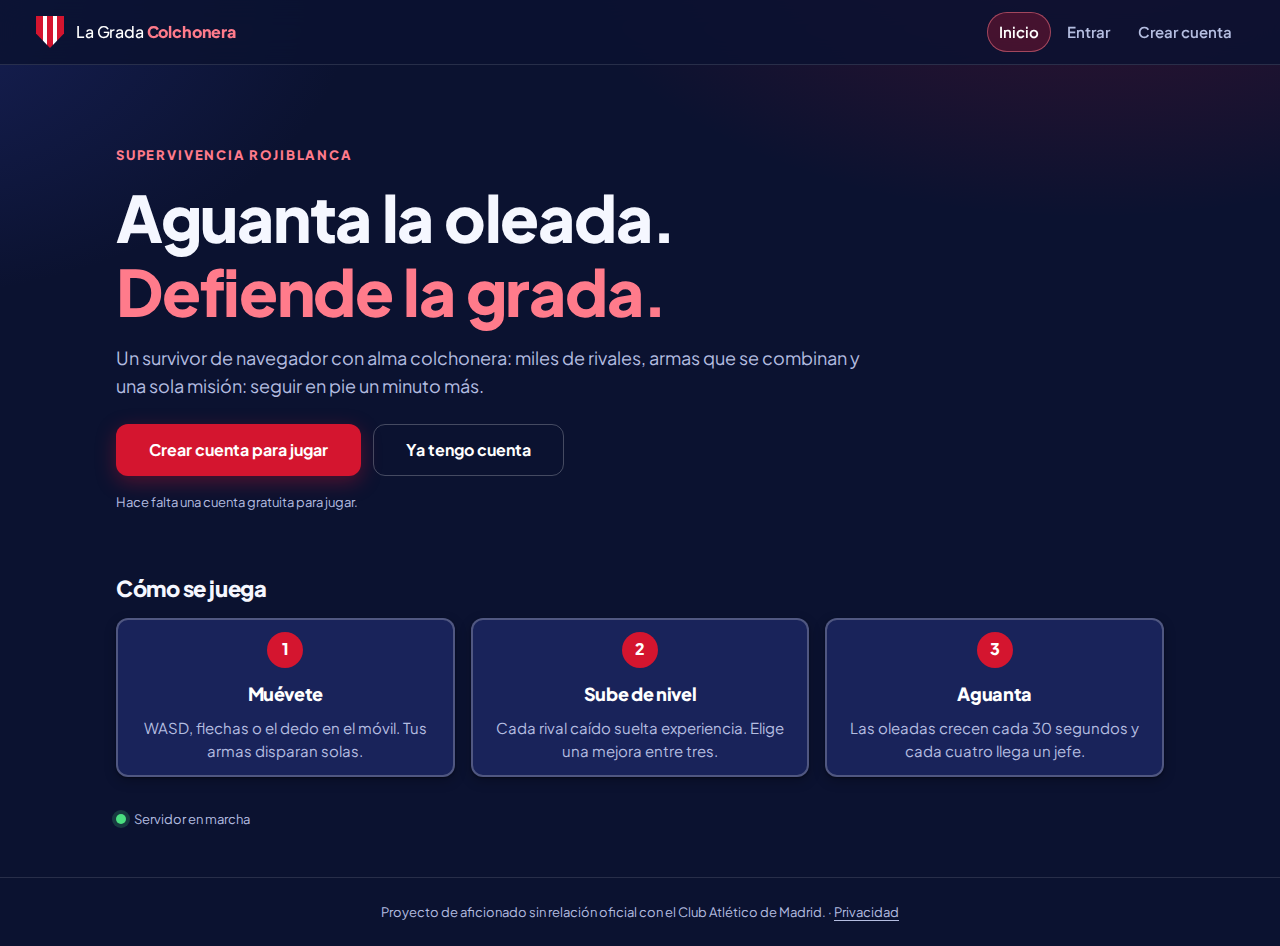
\includegraphics[width=0.9\textwidth]{figs/capturas/app/01-inicio.png}
\caption{Página de inicio sin sesión: botones para crear cuenta o entrar, cómo se juega y estado del servidor (P7).}
\label{fig:app-inicio}
\end{figure}

\begin{figure}[htbp]
\centering
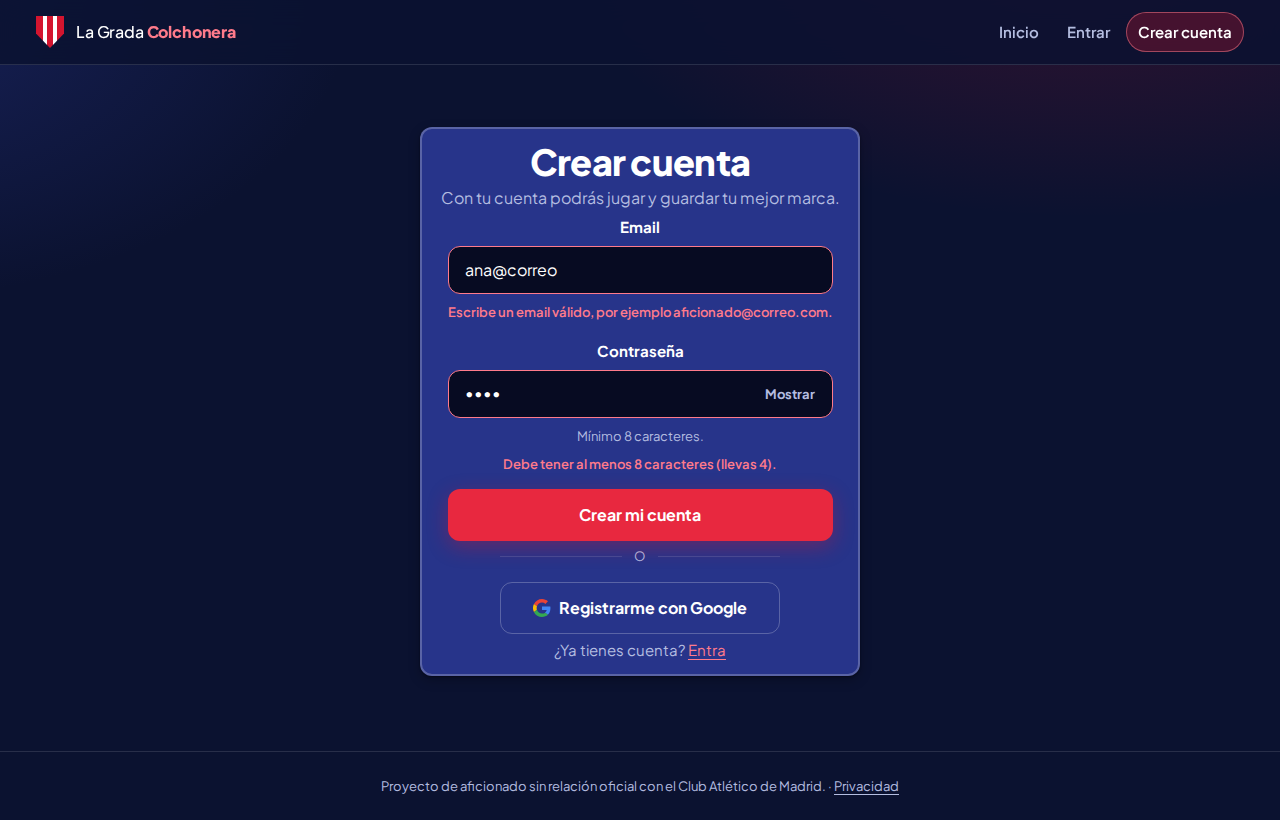
\includegraphics[width=0.9\textwidth]{figs/capturas/app/02-registro-validacion.png}
\caption{Registro con email y contraseña no válidos: campos en rojo y errores explicados (RF-01, RF-12).}
\label{fig:app-registro-val}
\end{figure}

\begin{figure}[htbp]
\centering
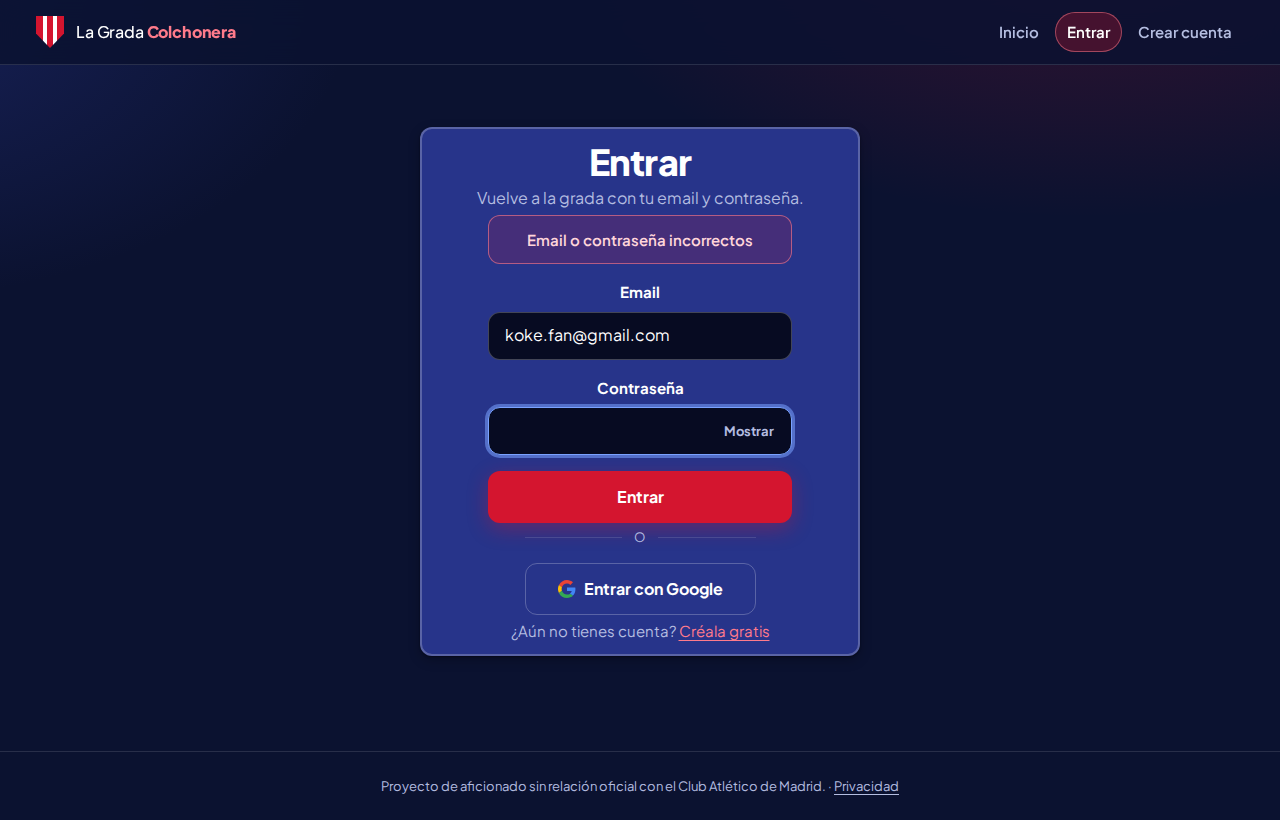
\includegraphics[width=0.9\textwidth]{figs/capturas/app/03-entrar-error.png}
\caption{Entrar con contraseña incorrecta: «Email o contraseña incorrectos» (RF-02, RF-12).}
\label{fig:app-login-err}
\end{figure}

\begin{figure}[htbp]
\centering
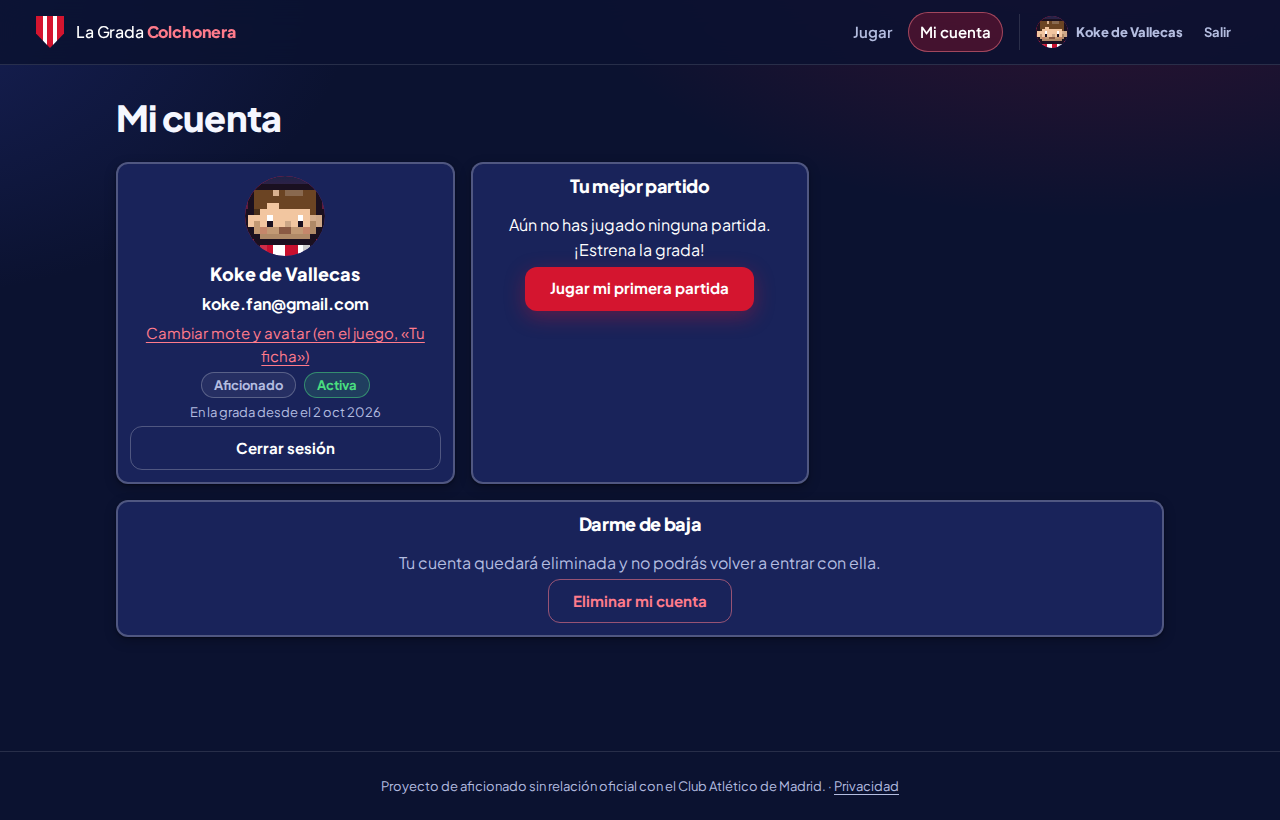
\includegraphics[width=0.9\textwidth]{figs/capturas/app/04-perfil.png}
\caption{Mi cuenta: mote, avatar, email, rol Aficionado, estado Activa, fecha de alta, cerrar sesión y darse de baja (RF-03, RF-08, RF-09).}
\label{fig:app-perfil}
\end{figure}

La Figura~\ref{fig:app-baja-conf} muestra el diálogo de confirmación antes de la baja. La Figura~\ref{fig:app-sin-permiso} ilustra la redirección de un usuario normal que intenta acceder a administración.

\begin{figure}[htbp]
\centering
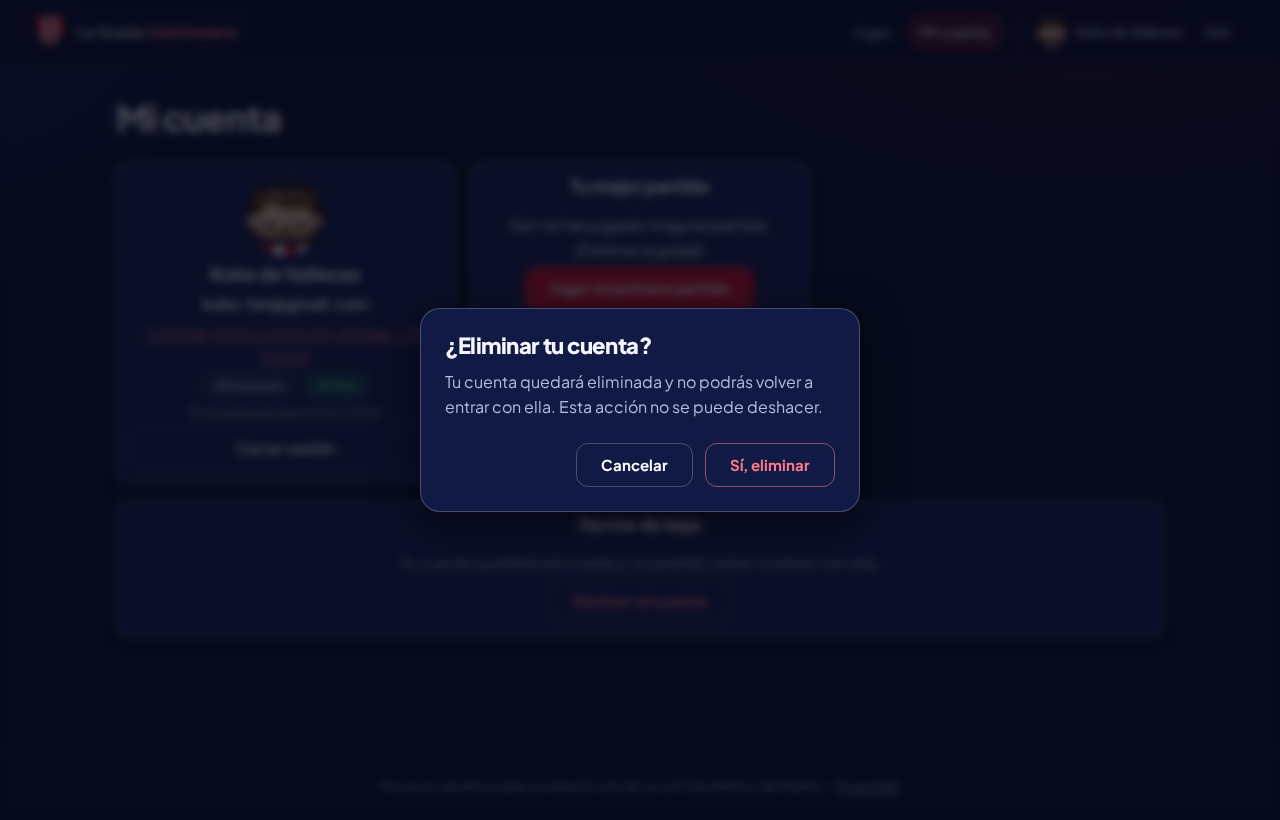
\includegraphics[width=0.9\textwidth]{figs/capturas/app/05-confirmar-baja.png}
\caption{Diálogo «¿Eliminar tu cuenta?» antes de darse de baja (RF-08, RF-12).}
\label{fig:app-baja-conf}
\end{figure}

\begin{figure}[htbp]
\centering
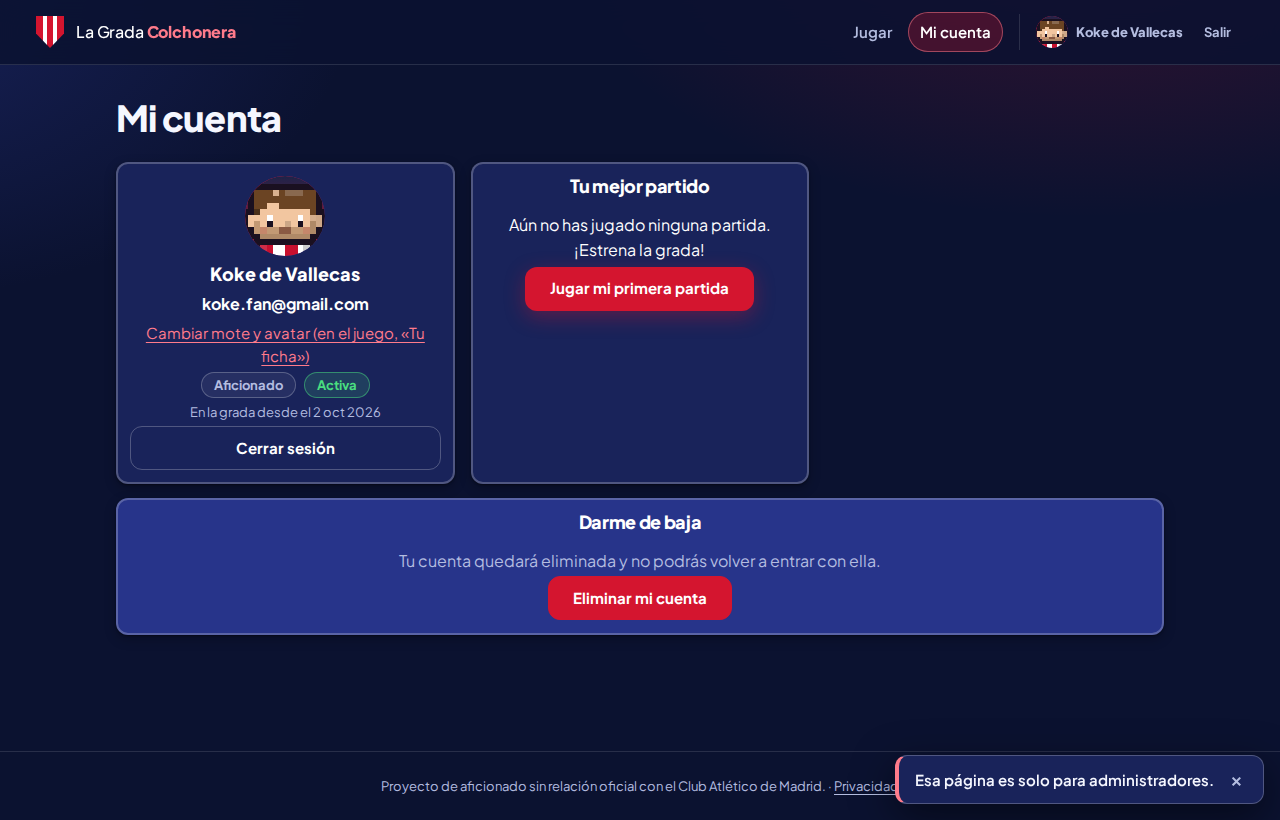
\includegraphics[width=0.9\textwidth]{figs/capturas/app/06-usuario-sin-permiso.png}
\caption{Usuario normal intenta abrir \texttt{\#/admin} y vuelve a Mi cuenta con aviso «Esa página es solo para administradores» (RF-04, RF-07).}
\label{fig:app-sin-permiso}
\end{figure}

\subsection{Panel de administración}

Las Figuras~\ref{fig:app-admin} a \ref{fig:app-admin-movil} muestran el panel de administración: listado con buscador, estados vacíos, confirmación de eliminación y vista responsive en móvil.

\begin{figure}[htbp]
\centering
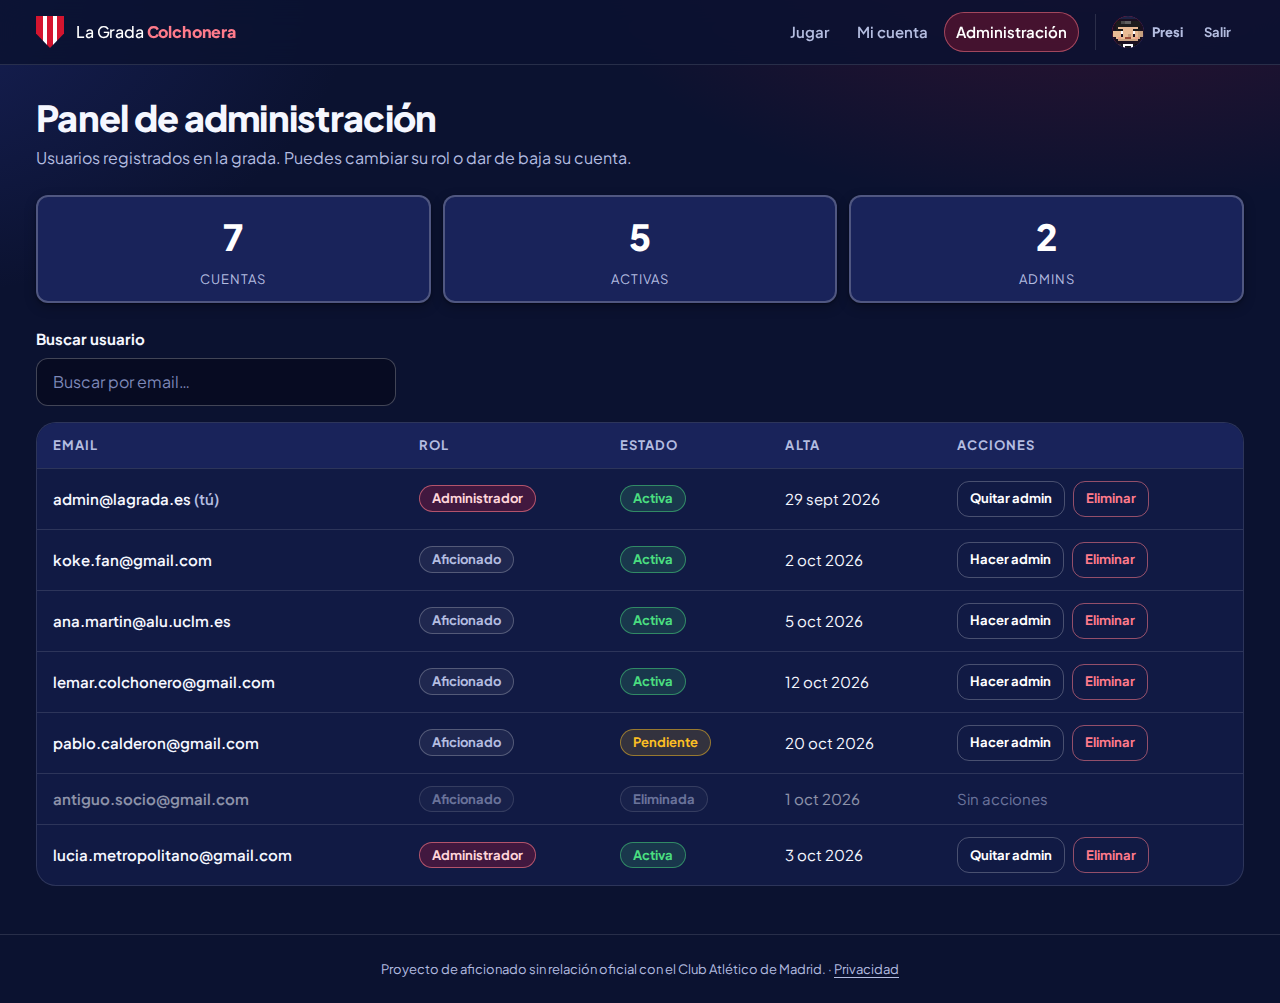
\includegraphics[width=0.9\textwidth]{figs/capturas/app/07-panel-admin.png}
\caption{Panel de administración: contadores, buscador y tabla con email, rol, estado, alta y acciones (RF-07).}
\label{fig:app-admin}
\end{figure}

\begin{figure}[htbp]
\centering
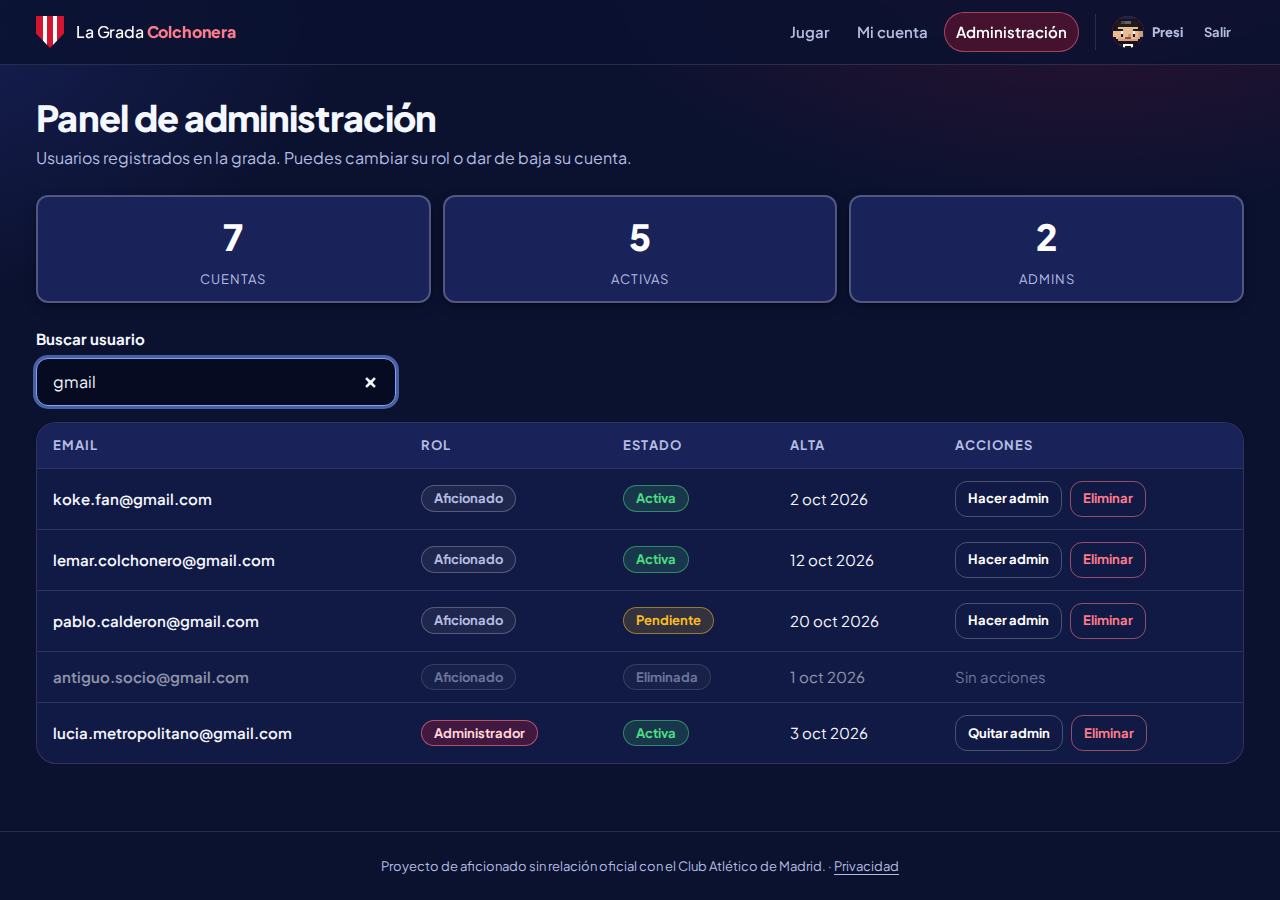
\includegraphics[width=0.9\textwidth]{figs/capturas/app/08-admin-busqueda.png}
\caption{Panel filtrado por email (RF-07).}
\label{fig:app-admin-busqueda}
\end{figure}

\begin{figure}[htbp]
\centering
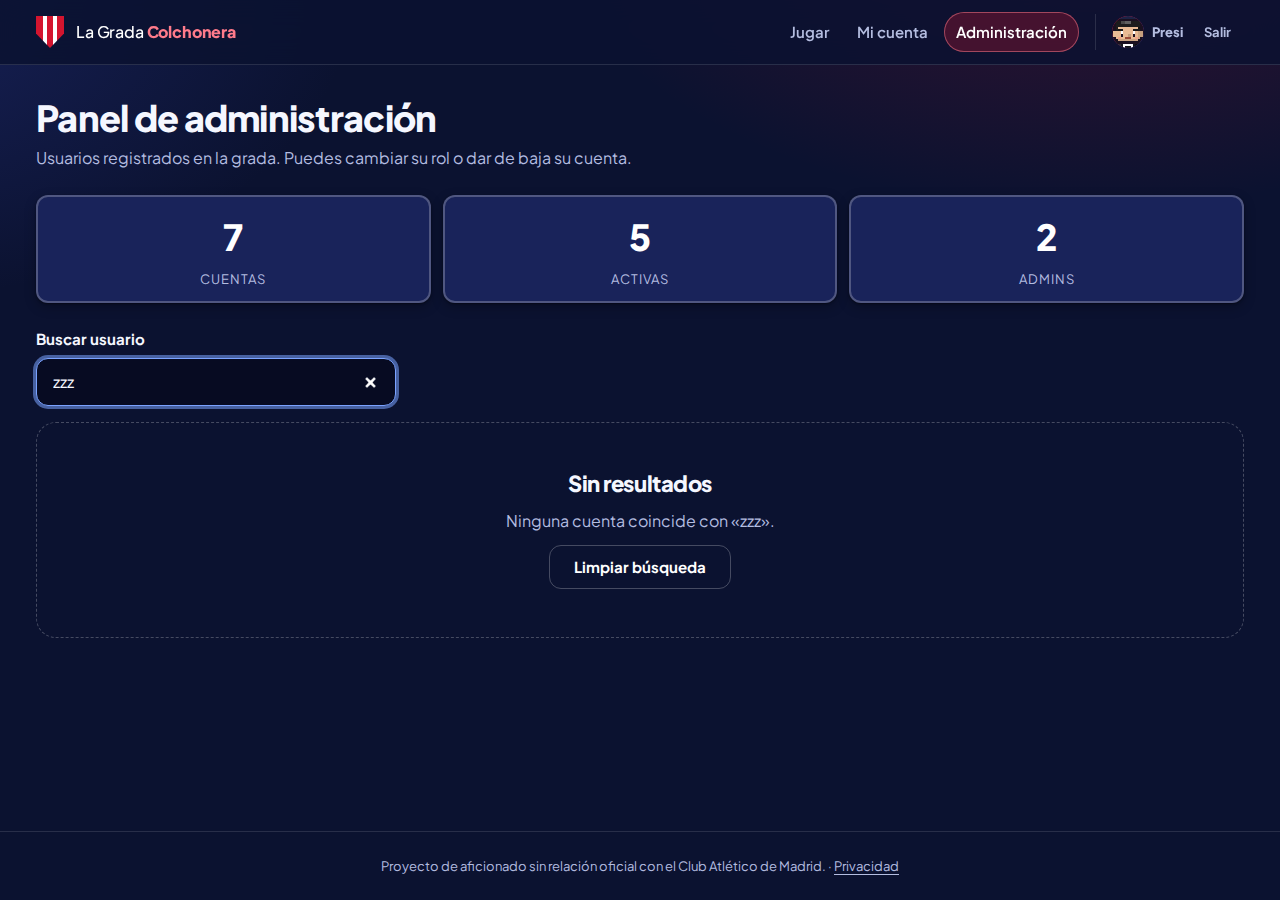
\includegraphics[width=0.9\textwidth]{figs/capturas/app/09-admin-sin-resultados.png}
\caption{Estado vacío de la búsqueda con botón «Limpiar búsqueda» (RF-12).}
\label{fig:app-admin-vacio}
\end{figure}

\begin{figure}[htbp]
\centering
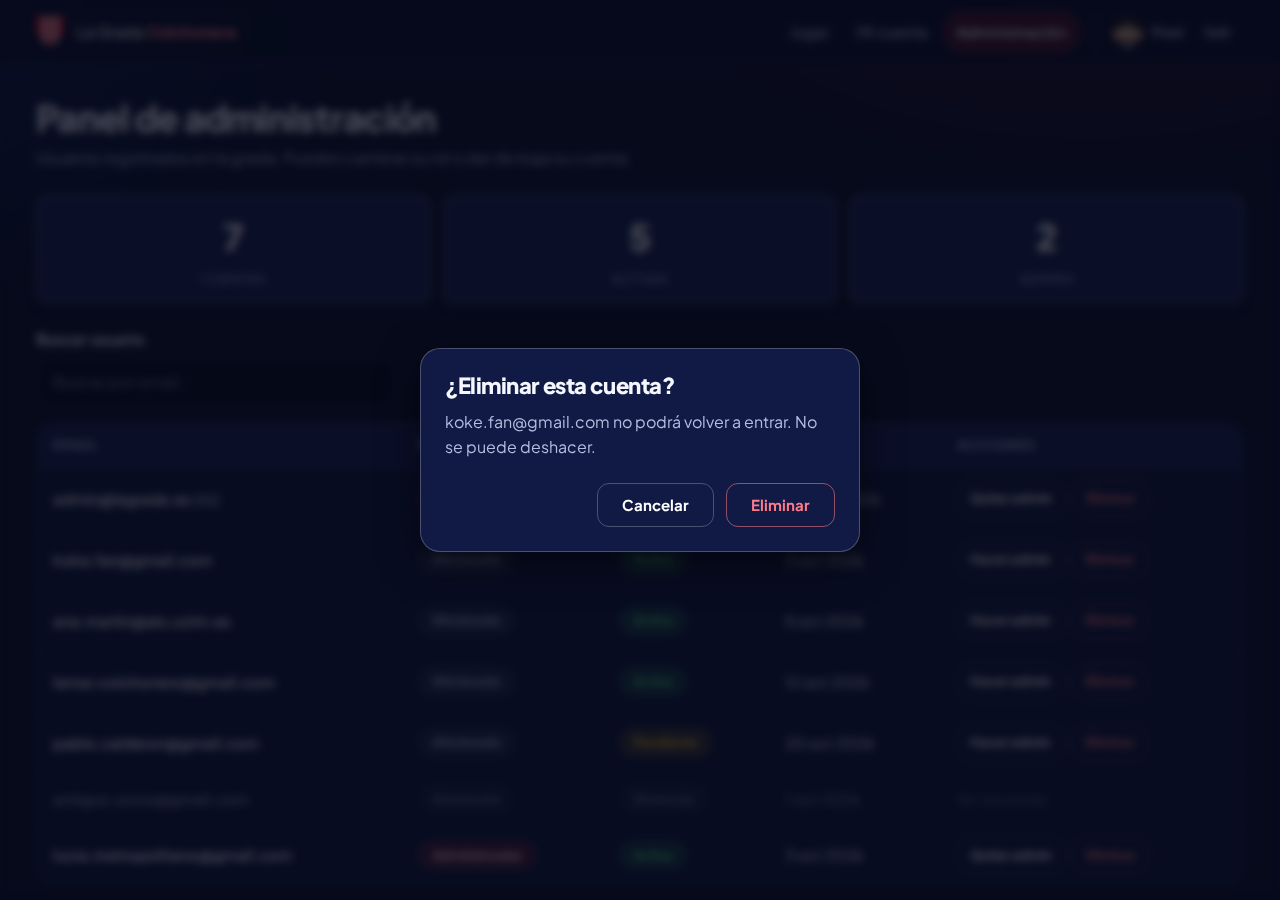
\includegraphics[width=0.9\textwidth]{figs/capturas/app/10-admin-confirmar-eliminar.png}
\caption{Diálogo de confirmación antes de eliminar otra cuenta desde el panel (RF-08).}
\label{fig:app-admin-del-conf}
\end{figure}

\begin{figure}[htbp]
\centering

\includegraphics[width=0.35\textwidth]{figs/capturas/app/11-panel-admin-movil.png}
\caption{Panel de administración en móvil: cada usuario es una tarjeta (RNF-08).}
\label{fig:app-admin-movil}
\end{figure}

\begin{figure}[htbp]
\centering

\includegraphics[width=0.35\textwidth]{figs/capturas/app/12-perfil-movil.png}
\caption{Mi cuenta en móvil con menú plegado (RNF-08).}
\label{fig:app-perfil-movil}
\end{figure}

\subsection{Hito 4: correo, Google y errores}

La Figura~\ref{fig:hito4-google} muestra el botón «Entrar con Google». La Figura~\ref{fig:hito4-correo-enviado} el aviso tras registro con correo de confirmación. Las Figuras~\ref{fig:hito4-pendiente-reenvio} y \ref{fig:hito4-reenvio} cubren el error de cuenta pendiente y el reenvío. Las Figuras~\ref{fig:hito4-enlace-invalido} y \ref{fig:hito4-confirmada} muestran enlace manipulado y confirmación exitosa. La Figura~\ref{fig:hito4-primer-acceso} el primer acceso tras confirmar. La Figura~\ref{fig:hito4-google-creada} la cuenta nueva por Google. La Figura~\ref{fig:hito4-error-reintento} el estado de error con botón Reintentar. La Figura~\ref{fig:hito4-admin-estados} el panel con todos los estados de cuenta. La Figura~\ref{fig:hito4-privacidad} la política de privacidad.

\begin{figure}[htbp]
\centering
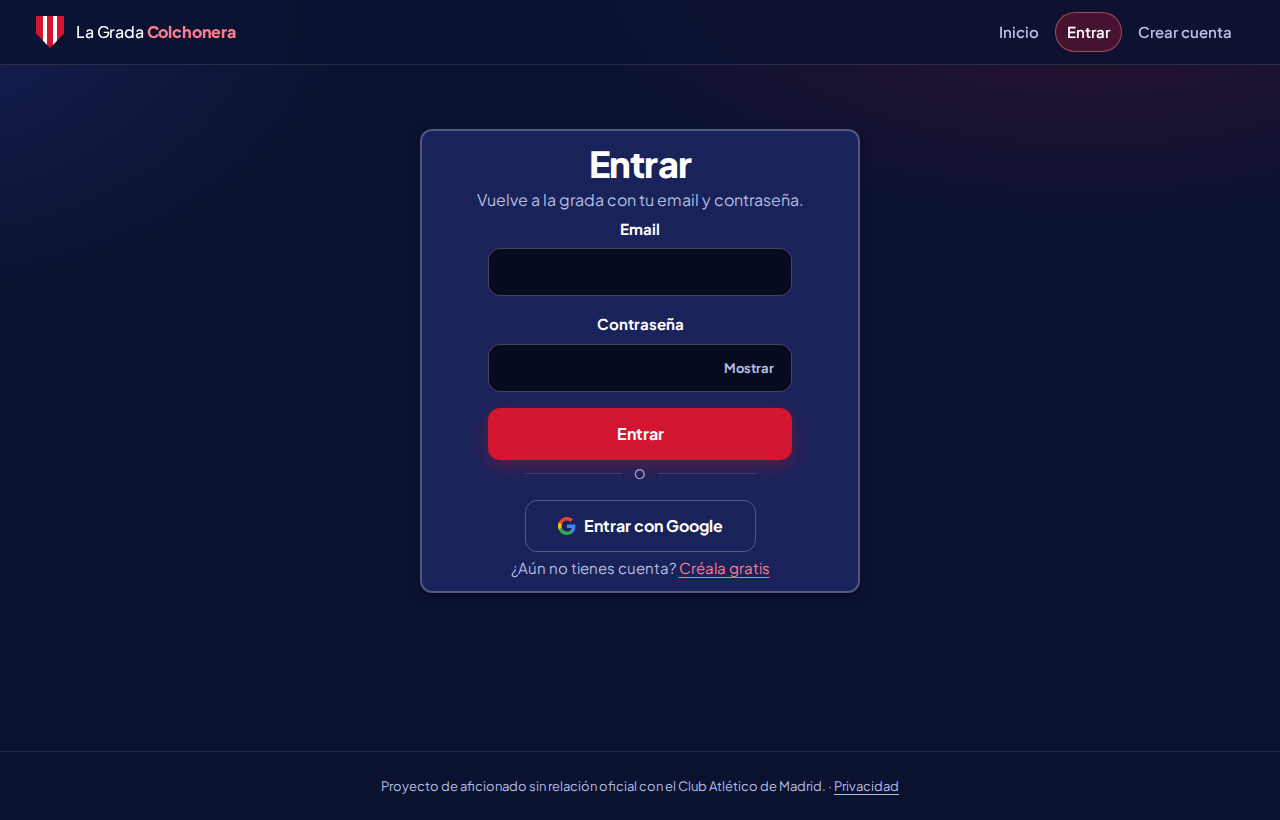
\includegraphics[width=0.9\textwidth]{figs/capturas/hito4/01-entrar-google.png}
\caption{Pantalla de entrar con el botón «Entrar con Google» (RF-11).}
\label{fig:hito4-google}
\end{figure}

\begin{figure}[htbp]
\centering
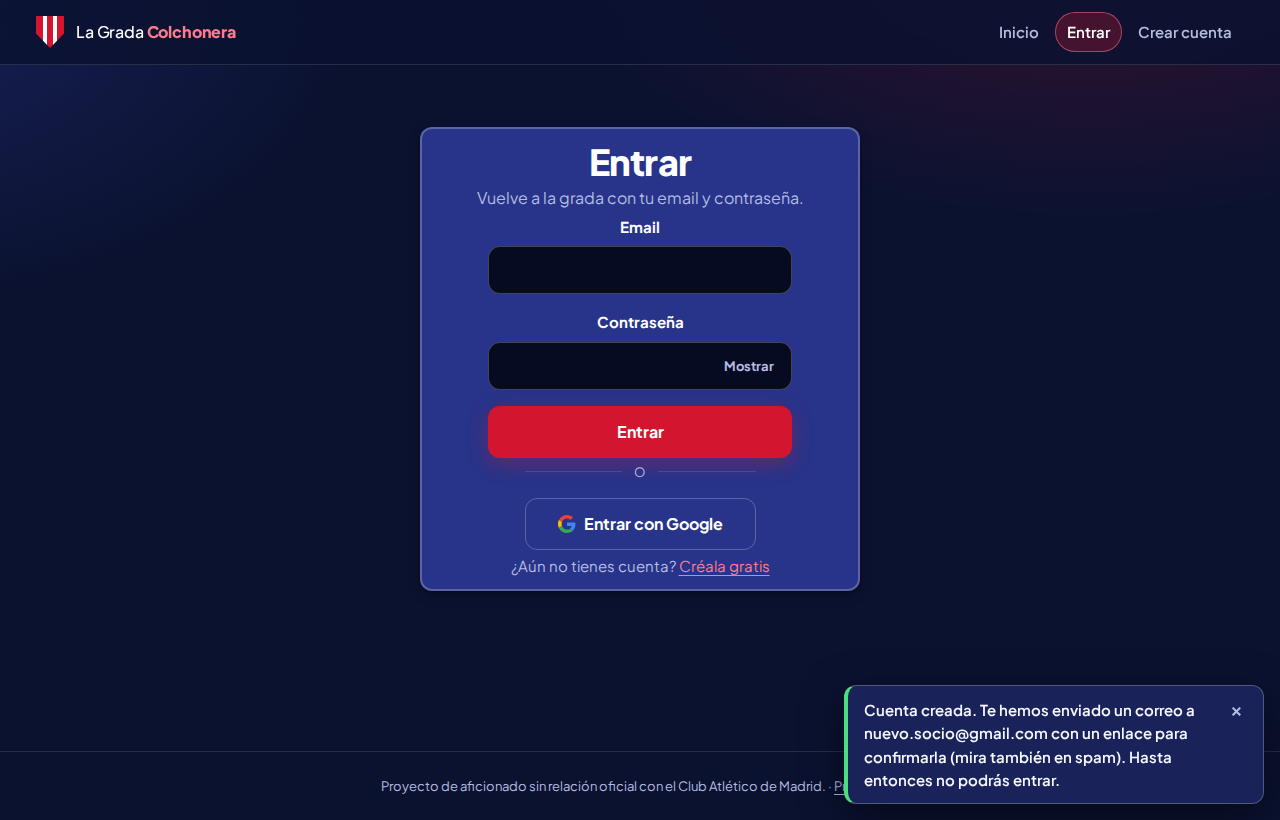
\includegraphics[width=0.9\textwidth]{figs/capturas/hito4/02-registro-correo-enviado.png}
\caption{Registro: aviso de cuenta creada y correo de confirmación enviado (RF-10).}
\label{fig:hito4-correo-enviado}
\end{figure}

\begin{figure}[htbp]
\centering
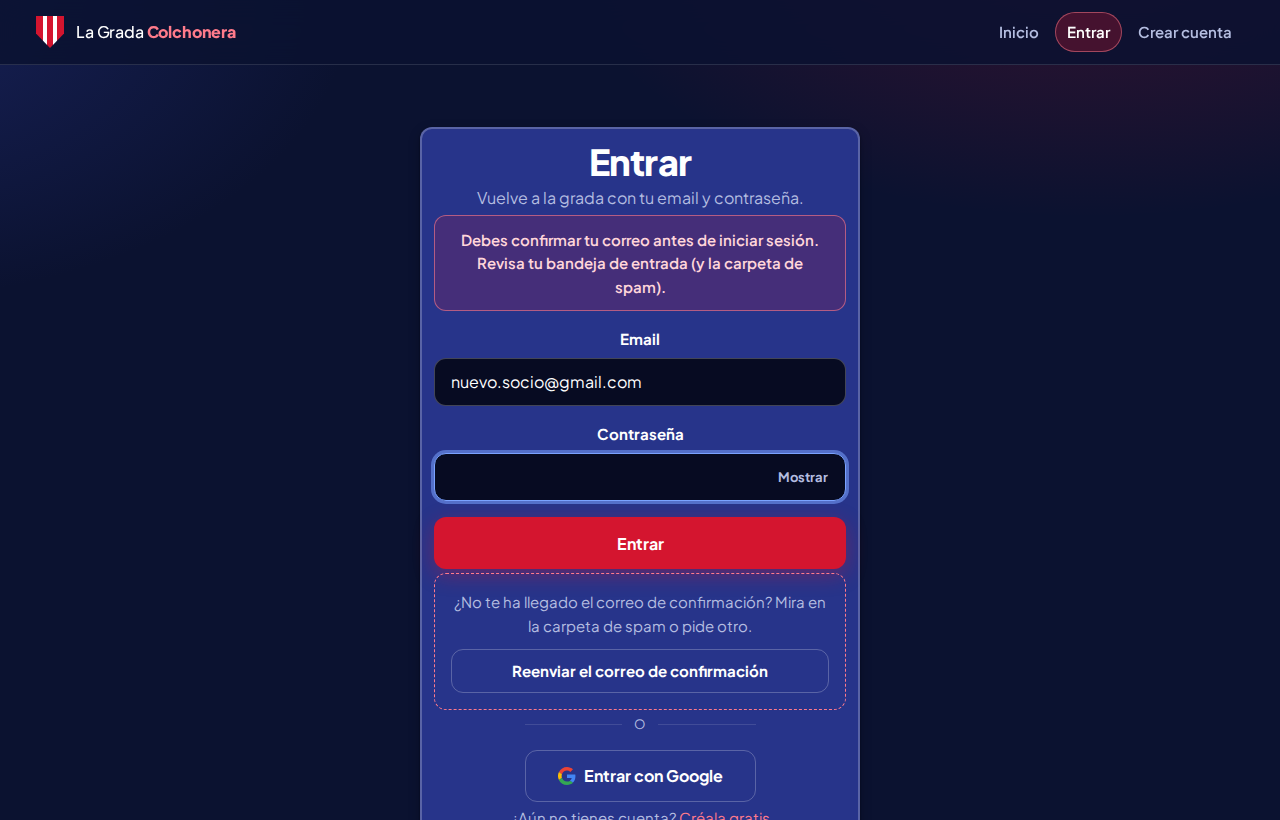
\includegraphics[width=0.9\textwidth]{figs/capturas/hito4/03-cuenta-pendiente-reenvio.png}
\caption{Login de cuenta pendiente: error y botón «Reenviar el correo de confirmación» (RF-10, RF-12).}
\label{fig:hito4-pendiente-reenvio}
\end{figure}

\begin{figure}[htbp]
\centering
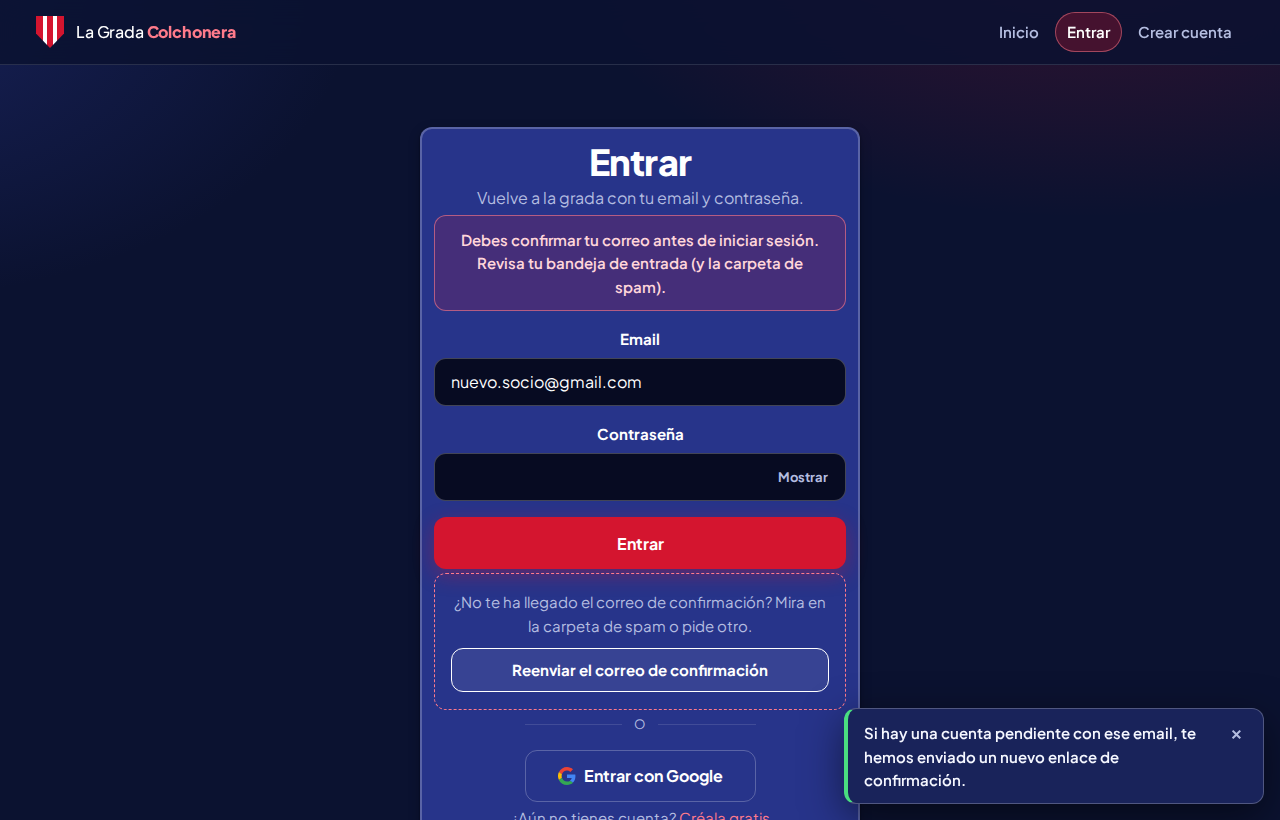
\includegraphics[width=0.9\textwidth]{figs/capturas/hito4/04-reenvio-hecho.png}
\caption{Aviso de reenvío (no revela si la cuenta existe) (RF-10).}
\label{fig:hito4-reenvio}
\end{figure}

\begin{figure}[htbp]
\centering
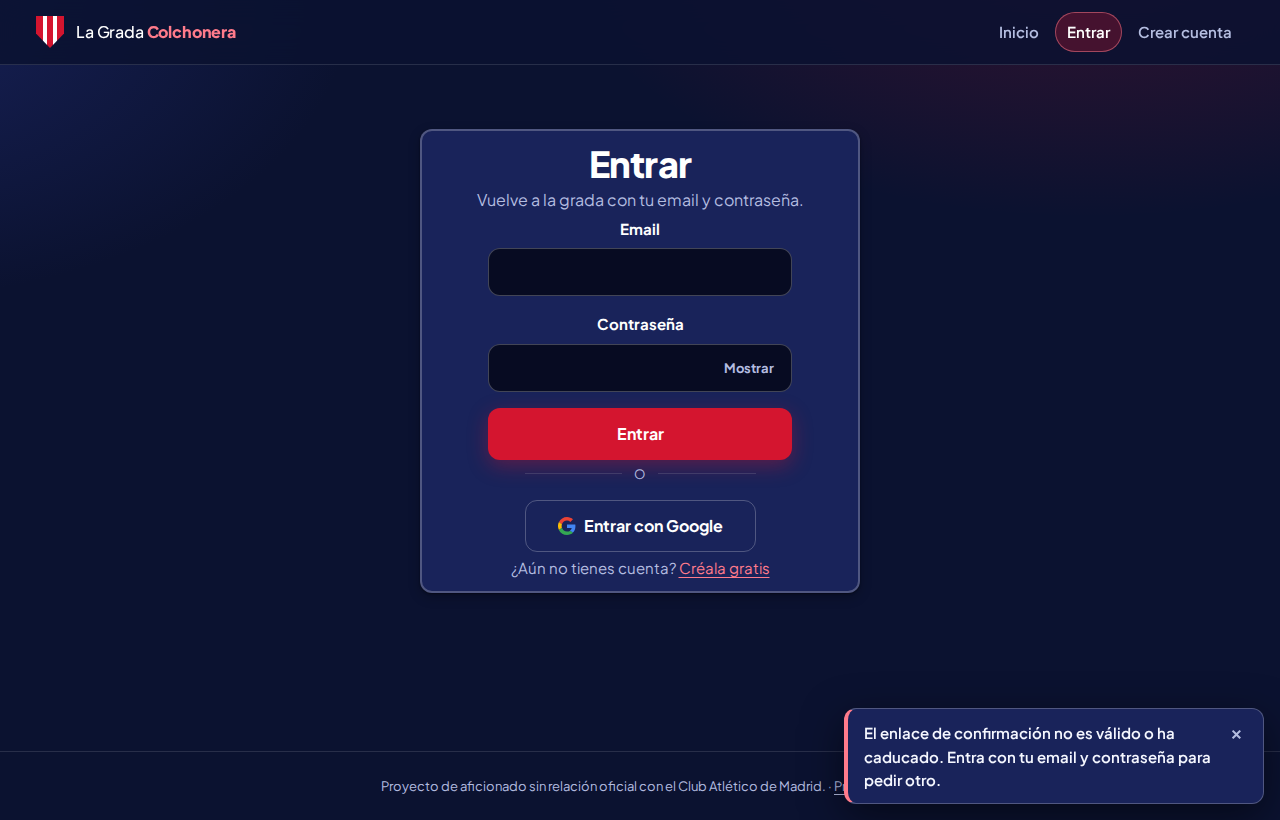
\includegraphics[width=0.9\textwidth]{figs/capturas/hito4/05-enlace-invalido.png}
\caption{Enlace manipulado o caducado: aviso rojo, la cuenta sigue pendiente (RF-10, RF-12).}
\label{fig:hito4-enlace-invalido}
\end{figure}

\begin{figure}[htbp]
\centering
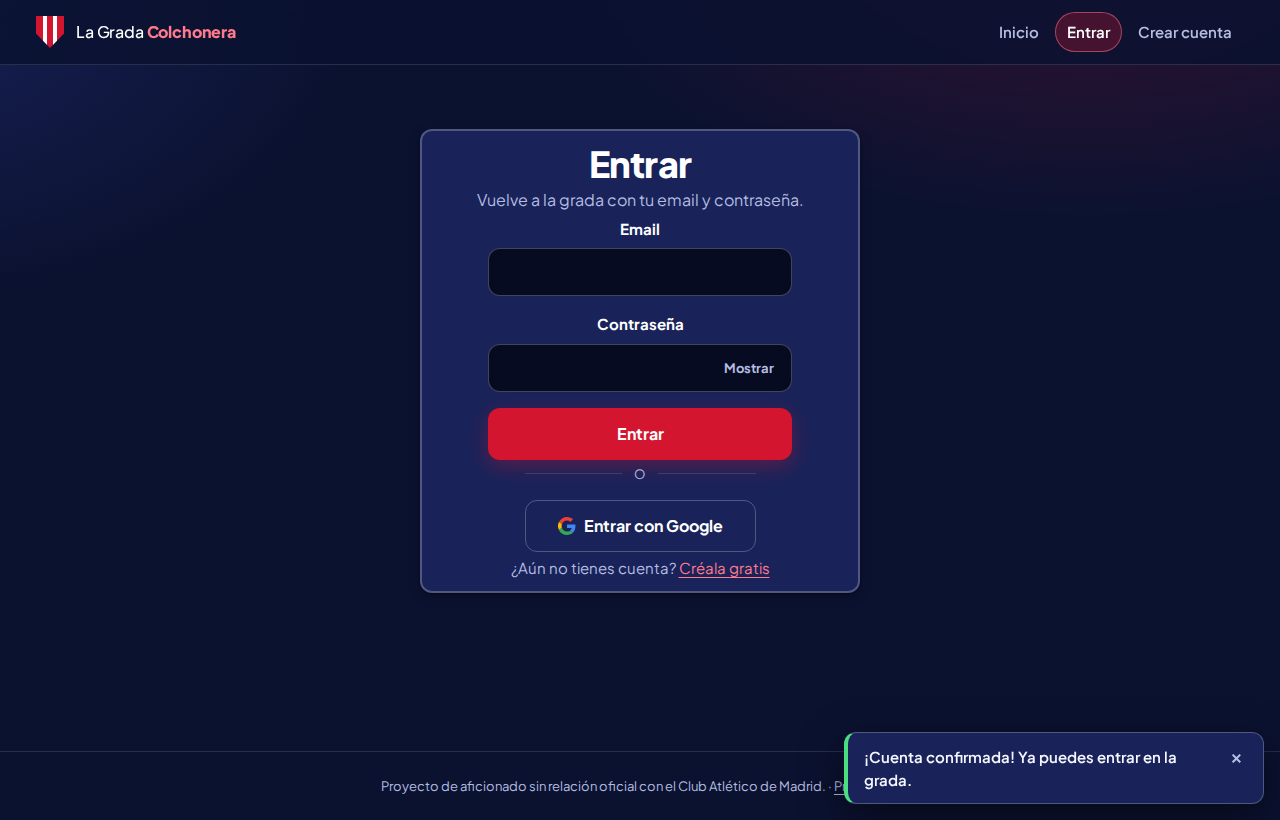
\includegraphics[width=0.9\textwidth]{figs/capturas/hito4/06-cuenta-confirmada.png}
\caption{Enlace correcto: aviso verde de cuenta confirmada (RF-10).}
\label{fig:hito4-confirmada}
\end{figure}

\begin{figure}[htbp]
\centering
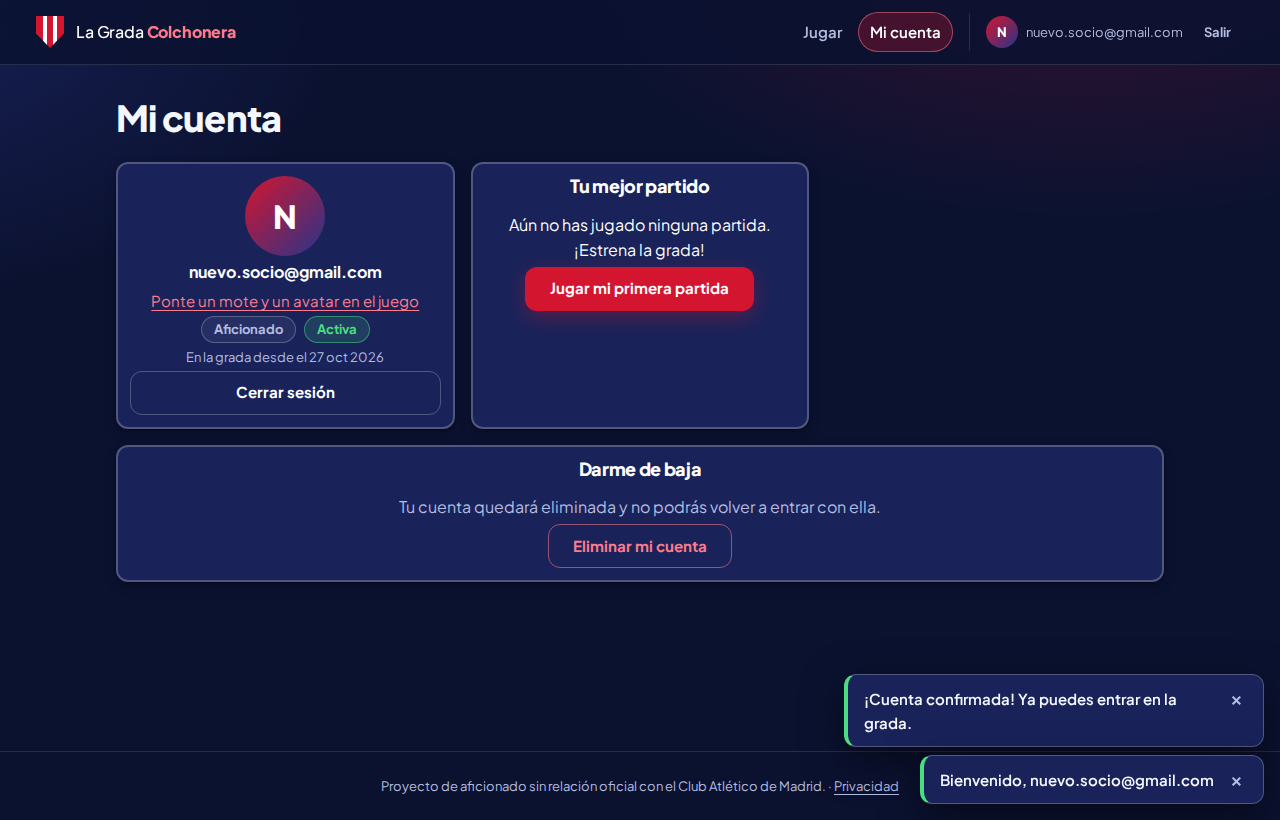
\includegraphics[width=0.9\textwidth]{figs/capturas/hito4/07-primer-acceso.png}
\caption{Primer acceso tras confirmar: Mi cuenta con aviso de bienvenida (RF-10).}
\label{fig:hito4-primer-acceso}
\end{figure}

\begin{figure}[htbp]
\centering
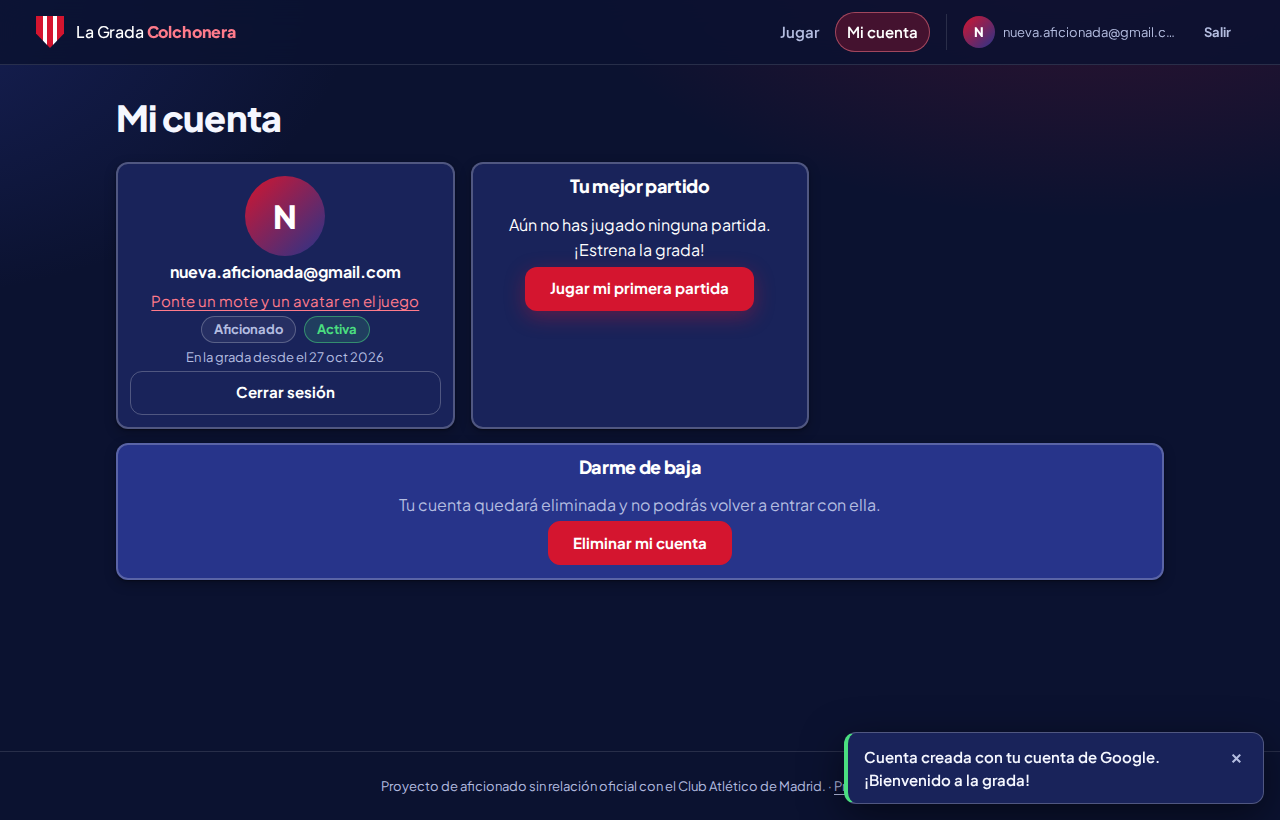
\includegraphics[width=0.9\textwidth]{figs/capturas/hito4/08-google-cuenta-creada.png}
\caption{Cuenta nueva con Google: Mi cuenta con aviso «Cuenta creada con tu cuenta de Google» (RF-11).}
\label{fig:hito4-google-creada}
\end{figure}

\begin{figure}[htbp]
\centering
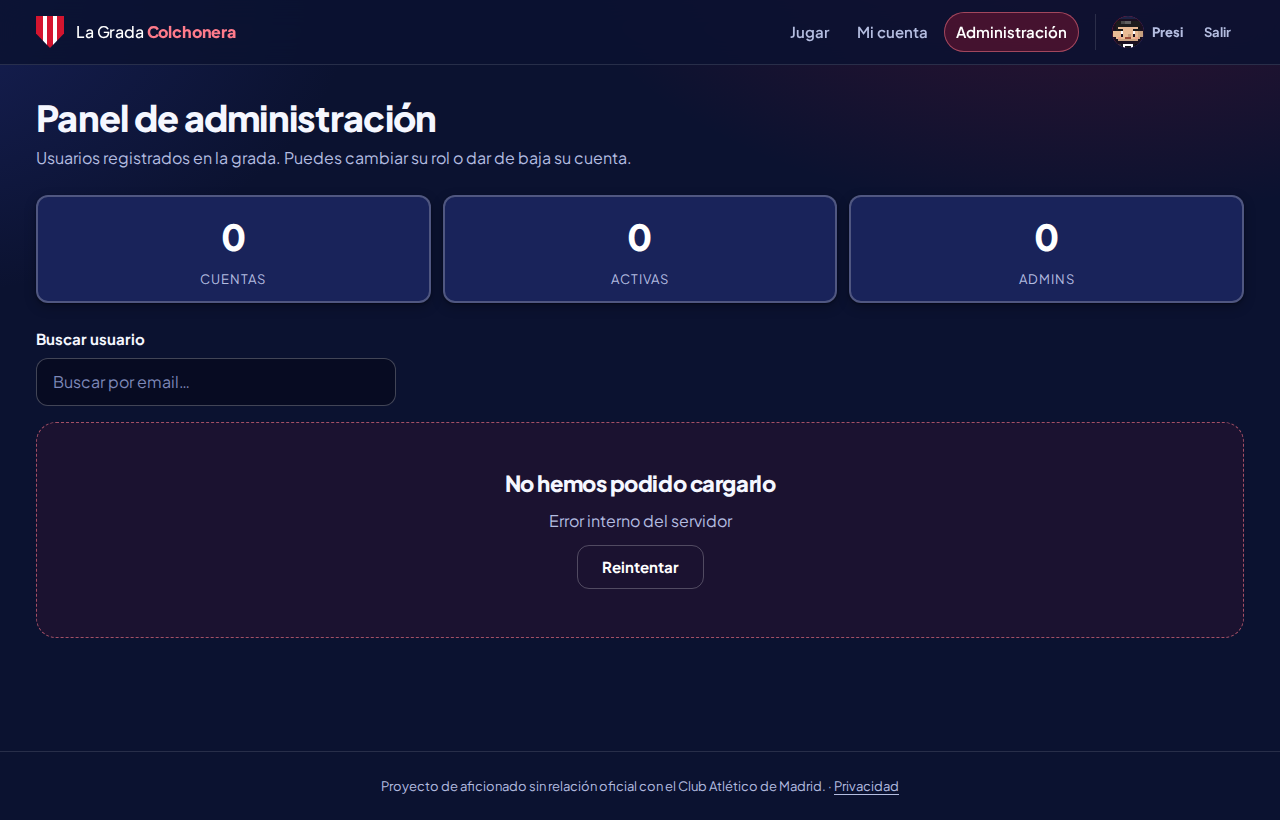
\includegraphics[width=0.9\textwidth]{figs/capturas/hito4/09-error-con-reintento.png}
\caption{Fallo del servidor al cargar el panel: «No hemos podido cargarlo» con botón Reintentar (RF-12).}
\label{fig:hito4-error-reintento}
\end{figure}

\begin{figure}[htbp]
\centering
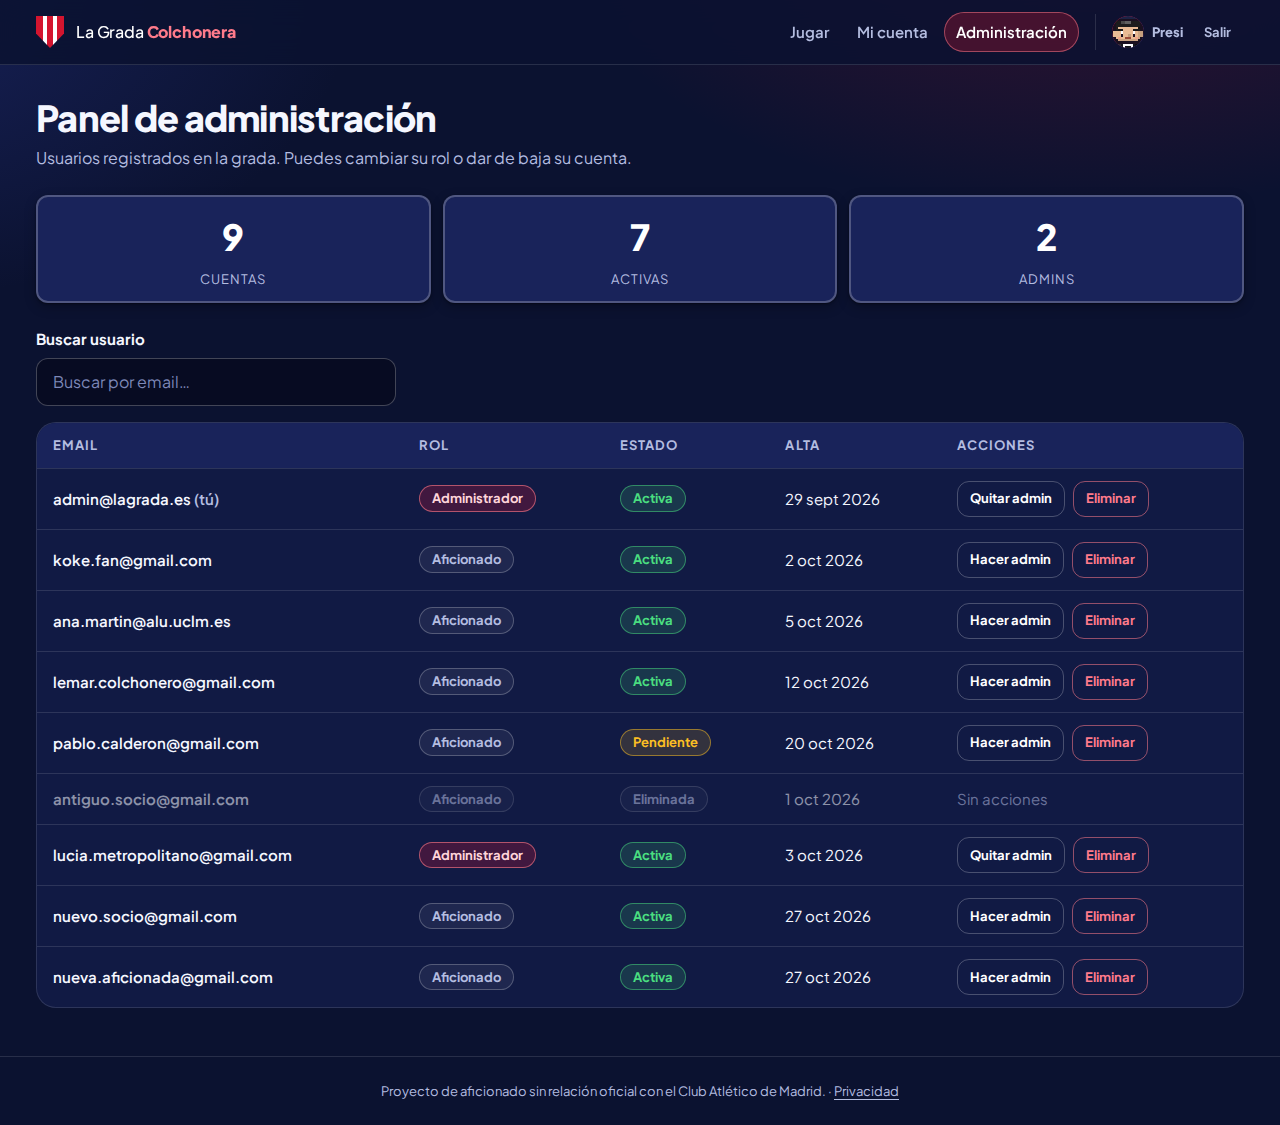
\includegraphics[width=0.9\textwidth]{figs/capturas/hito4/10-panel-admin-estados.png}
\caption{Panel con cuentas activas, pendientes, eliminadas, locales y de Google (RF-07, RF-11, RF-10).}
\label{fig:hito4-admin-estados}
\end{figure}

\begin{figure}[htbp]
\centering

\includegraphics[width=0.9\textwidth]{figs/capturas/hito4/11-privacidad.png}
\caption{Política de privacidad (RNF-11).}
\label{fig:hito4-privacidad}
\end{figure}

La ruta inexistente muestra «Fuera de juego» (Figura~\ref{fig:app-404}).

\begin{figure}[htbp]
\centering
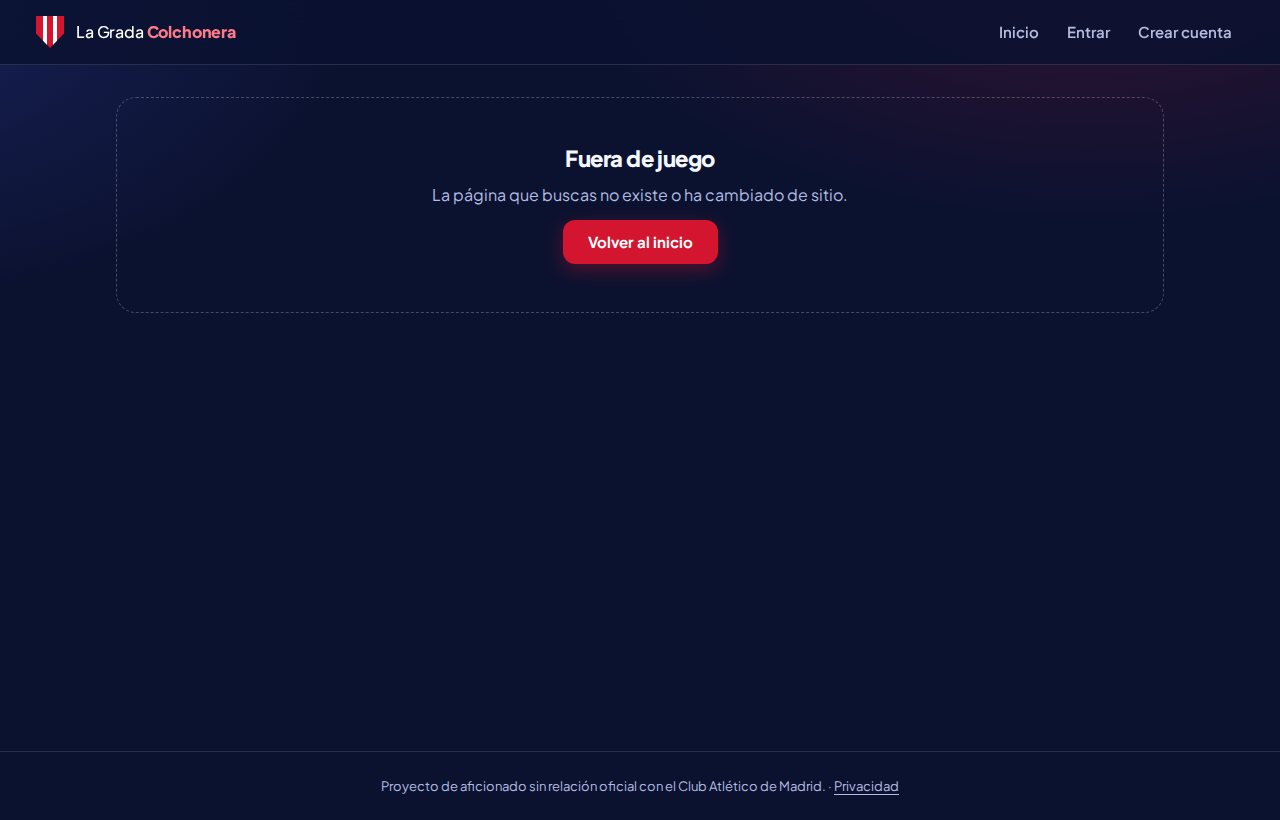
\includegraphics[width=0.9\textwidth]{figs/capturas/app/13-pagina-no-encontrada.png}
\caption{Ruta inexistente: «Fuera de juego» (RF-12).}
\label{fig:app-404}
\end{figure}

Todas las capturas proceden de \texttt{figs/capturas/app/} y \texttt{figs/capturas/hito4/} (documentacion-tecnica.md §16). El subsistema SaaS queda así completamente documentado; el juego se detalla en el Capítulo~\ref{cap:juego}.
